\documentclass[journal]{style/vgtc} 			          % final (journal style)
%\documentclass[review,journal]{style/vgtc}         % review (journal style)
%\documentclass[widereview]{style/vgtc}             % wide-spaced review
%\documentclass[preprint,journal]{style/vgtc}       % preprint (journal style)
%\documentclass[electronic,journal]{style/vgtc}     % electronic version, journal

%% Uncomment one of the lines above depending on where your paper is
%% in the conference process. ``review'' and ``widereview'' are for review
%% submission, ``preprint'' is for pre-publication, and the final version
%% doesn't use a specific qualifier. Further, ``electronic'' includes
%% hyperreferences for more convenient online viewing.

%% Please use one of the ``review'' options in combination with the
%% assigned online id (see below) ONLY if your paper uses a double blind
%% review process. Some conferences, like IEEE Vis and InfoVis, have NOT
%% in the past.

%% Please note that the use of figures other than the optional teaser is not permitted on the first page
%% of the journal version.  Figures should begin on the second page and be
%% in CMYK or Grey scale format, otherwise, colour shifting may occur
%% during the printing process.  Papers submitted with figures other than the optional teaser on the
%% first page will be refused.

%% These three lines bring in essential packages: ``mathptmx'' for Type 1
%% typefaces, ``graphicx'' for inclusion of EPS figures. and ``times''
%% for proper handling of the times font family.

\usepackage{mathptmx}
\usepackage{graphicx}
\usepackage{times}

%% We encourage the use of mathptmx for consistent usage of times font
%% throughout the proceedings. However, if you encounter conflicts
%% with other math-related packages, you may want to disable it.

%% This turns references into clickable hyperlinks.
\usepackage[bookmarks,backref=true,linkcolor=black]{hyperref} %,colorlinks
\hypersetup{
  pdfauthor = {},
  pdftitle = {},
  pdfsubject = {},
  pdfkeywords = {},
  colorlinks=true,
  linkcolor= black,
  citecolor= black,
  pageanchor=true,
  urlcolor = black,
  plainpages = false,
  linktocpage
}

%% If you are submitting a paper to a conference for review with a double
%% blind reviewing process, please replace the value ``0'' below with your
%% OnlineID. Otherwise, you may safely leave it at ``0''.
\onlineid{0}

%% declare the category of your paper, only shown in review mode
\vgtccategory{Research}

%% allow for this line if you want the electronic option to work properly
\vgtcinsertpkg

%% In preprint mode you may define your own headline.
%\preprinttext{To appear in an IEEE VGTC sponsored conference.}

%% Paper title.

\title{Interactive Visual Analysis of Image-Centric Cohort Study Data}

%% This is how authors are specified in the journal style

%% indicate IEEE Member or Student Member in form indicated below
\author{--blind--}
\authorfooter{
%% insert punctuation at end of each item
% \item
%  Otto-v.-Guericke-University Magdeburg
}

%other entries to be set up for journal
\shortauthortitle{Klemm \MakeLowercase{\textit{et al.}}: Interactive Visual Analysis of Image-Centric Cohort Study Data}
%\shortauthortitle{Firstauthor \MakeLowercase{\textit{et al.}}: Paper Title}

%% Abstract section.
\abstract{%
%(The problem). 
Epidemiological population studies impose information about a set of subjects (a \emph{cohort}) to characterize disease-specific risk factors.
%
Cohort studies comprise heterogenous variables (\emph{features}) describing the medical condition as well as demographic and lifestyle factors.
%
The data is analyzed using a priori defined hypotheses to find statistically significant correlations between variables (\emph{interactions}).
%
Modern cohort studies also incorporate medical image data.
%
%Analyzing these data requires image segmentation, extraction of key figures, and shape based subject grouping.
%
The statistically driven epidemiological workflow only allows to determine \emph{interactions} between image-derived metrics such as distances extracted from landmarks of the segmentation model.
\\\\
%(New Solution).
We propose an Interactive Visual Analysis approach that enables epidemiologists to examine both image-based as well as non-image data, e.g., sociodemographic variables and attributes derived from the image data.
%
This is achieved by combining brushing and linking enabled coordinated information visualization views and interactive 3D shape renderings with epidemiological data representations such as pivot tables and key figures as association measures.
%incorporating coordinated views from information visualization and 3D-shape renderings are combined with epidemiological data representations such as Pivot Tables.
%
%Multiple coordinated views from information visualization and 3D-shape renderings are combined with epidemiological data representations such as Pivot Tables.
%
%(Validation).
The presented concepts are applied expert-guided to gather and evaluate hypotheses about the aging process of the lumbar spine.
%
%(Results). 
It shows to be a more flexible comparison between image and non-image data.
%
%(Implications).
The new framework allows for hypothesis validation and hypothesis generation by incorporating human pattern recognition as well as data mining methods.
%
Using all reliable information from the image segmentation linked to non-image variables aims to unveil \emph{interactions} by applying an iterative analysis approach.

%
%Similarity measures between data variables are used to compute interesting changes in variable interactions for the current variable selection.
%
%Shape based grouping of subjects is facilitated using clustering techniques which operate on surface meshes extracted from the image segmentation.
} % end of abstract

% \abstract{Epidemiological population studies impose information about a set of subjects (a \emph{cohort}) to characterize disease specific risk factors.
% %
% Cohort studies comprise heterogenous variables (\emph{features}) describing the medical condition as well as demographic and lifestyle factors.
% %
% %Using well established statistical methods the data is hypothesis driven analyzed to find statistically significant variable correlations (\emph{interactions}).
% Driven by a priori defined hypotheses, the data is analyzed using well established statistical methods in order to find statistically significant correlations between variables (\emph{interactions}).
% %
% Modern cohort studies also incorporate medical image data.
% %
% Analyzing these data requires image segmentation, extraction of key figures, and shape based subject grouping.
% %
% The statistically driven epidemiological workflow only allows to determine \emph{interactions} between image-derived metrics such as distances extracted from landmarks of the segmentation model.
% \\\\
% We propose an Interactive Visual Analysis approach that enables epidemiologists to examine both image-based as well as non-image data, e.g., sociodemographic variables and attributes derived from the image data.
% %
% Using all reliable information from the image segmentation linked to non-image variables aims to unveil \emph{interactions} by applying an iterative analysis approach.
% %As extension to the epidemiological workflow it aims to unveil interactions based on all reliable shape information rather than abstracting it to a few key figures.
% %Iterative analysis between ... allows for extracting interactions which without the visiual analysis driven approach maybe would be overlooked. %Einsicht in Interaktionen zwischen nicht-bilddaten und bilddaten auf basis aller verfügbarer Informationen 
% %Iterative Analyse von Organstrukturen im Bezug auf Bilddaten 
% %Iterative analysis of image-based epidemiological datasets aims to provide insight into interactions between organ shape and % in order to provide insights into \emph{interactions} by incorporating additional information
% %It extends the epidemiological workflow with an iterative Analysis process and 
% It allows for hypothesis validation and hypothesis generation by incorporating human pattern recognition as well as data mining methods.
% %
% Multiple coordinated views from information visualization and 3D-shape renderings are combined with epidemiological data representations such as Pivot Tables.
% %
% Similarity measures between data variables are used to compute interesting changes in variable interactions for the current variable selection.
% %
% Shape based grouping of subjects is facilitated using clustering techniques which operate on surface meshes extracted from the image segmentation.
% } % end of abstract


%% Keywords that describe your work. Will show as 'Index Terms' in journal
%% please capitalize first letter and insert punctuation after last keyword
\keywords{Interactive Visual Analysis, Epidemiology, Spine}

%% ACM Computing Classification System (CCS). 
%% See <http://www.acm.org/class/1998/> for details.
%% The ``\CCScat'' command takes four arguments.

\CCScatlist{ % not used in journal version
 \CCScat{K.6.1}{Management of Computing and Information Systems}%
{Project and People Management}{Life Cycle};
 \CCScat{K.7.m}{The Computing Profession}{Miscellaneous}{Ethics}
}

%% Uncomment below to include a teaser figure.
  % \teaser{
  % \centering
  % \includegraphics[width=16cm]{CypressView}
  % \caption{In the Clouds: Vancouver from Cypress Mountain.}
  % }

%% Uncomment below to disable the manuscript note
%\renewcommand{\manuscriptnotetxt}{}

%% Copyright space is enabled by default as required by guidelines.
%% It is disabled by the 'review' option or via the following command:
% \nocopyrightspace

%%%%%%%%%%%%%%%%%%%%%%%%%%%%%%%%%%%%%%%%%%%%%%%%%%%%%%%%%%%%%%%%
%%%%%%%%%%%%%%%%%%%%%% START OF THE PAPER %%%%%%%%%%%%%%%%%%%%%%
%%%%%%%%%%%%%%%%%%%%%%%%%%%%%%%%%%%%%%%%%%%%%%%%%%%%%%%%%%%%%%%%%

\begin{document}

%% The ``\maketitle'' command must be the first command after the
%% ``begin{document}'' command. It prepares and prints the title block.

%% the only exception to this rule is the \firstsection command
\firstsection{Introduction}

\maketitle

%% \section{Introduction} %for journal use above \firstsection{..} instead
\textbf{(Background)} Epidemiology aims at characterizing health and disease by determining risk factors.
%
Clinical problems, such as the selection of diagnostic tools and efficient treatment, are tackled using results of epidemiological research.
%
Also, the introduction of preventive measures in medicine and beyond, are based on epidemiological research, where, for example, subgroups with increased risk are identified \cite{Fletcher2012}.
%
On the other hand, observations made by clinicians in the daily routine are translated into hypothesis for epidemiological research.
%
These are used to determine environmental and lifestyle factors as well as medical attributes which may influence a condition of interest.
%
The data variables necessary are gathered using structured interviews and clinical examinations.
%
Statistical methods like regression analysis aim to check the attribute list for plausibility.
%
\\\\
\textbf{(Problem)}
Longitudinal population-based studies, such as the Study of Health in Pomerania (SHIP) \cite{Volzke2011}, aim to gather as much information as possible about a defined sample of people (a \emph{cohort}).
%
% The sample is drawn randomized to avoid selection \cite{Fletcher2012}.
% %
% When for example one investigates risk factors for prostate cancer in male subjects, the outcome is strongly dependent on the age.
% %
% Therefore results need to be age-adjusted to be comparable.
% %
% Confounding variables, are often not obvious at all and characterizing them is already an epidemiological result.
%
Modern cohort studies often include medical image data.
%
These data needs to be segmented to analyze its features for correlations with non-image data.
%
Manual segmentation is not feasible since it leads to a high variability which is at odds with the high reproducibility required in epidemiology research.
%
Semi-automatic techniques are more promising but challenging since the used methods as MRI and ultrasound are subject to inhomogeneity and noise.
%
Analyzing spatial data with respect to other epidemiological factors requires techniques which reach beyond standard statistical methods.

Compiling a list of features for tests of statistical resilience based on experience-driven hypotheses leaves out other features in the data which potentially interact with a disease.
%
This also applies to the chosen landmarks which are used to quantify medical image data information.
%
The standard workflow lacks methods which highlight features of interest the epidemiologists did not consider.
%The hypothesis driven analysis approach of these data based on expectations of epidemiologists leaves out features which potentially interact with a disease outside.
%The hypothesis driven analysis approach of these data leaves out features which potentially interact with a disease because they they are it is outside of the erwartungshaltung of the epidemiologists.
%leaves out features which potentially interact with a disease because they are usually outside of the practical experience of the epidemiologists.
%
%Analyzing these data for correlating features requires preprocessing steps as segmentation of the structures.
%
%Manual segmentation is not feasible since it leads to a high variability which is att odds with the high reproducibility required in epidemiology research. 
%
%Semi-automatic techniques are more promising but challenging since MRI and ultrasound are subject to inhomogeneity and noise
%Due to the lack of sophisticated segmentation algorithms this is often achieved by manually specifying landmarks by radiologists which is costly and prone to inter- and intra observer variability.
%
% Since it is unethical to expose people to radiation, non-harming imaging such as Magnetic Resonance Imaging (MRI) or Ultrasound Imaging is used.
% %
% To quantify these data it is necessary to label each voxel regarding structure affiliation (\emph{segmentation}).
% %
% Manual segmentation carried out by radiological experts is possible but very costly and prone to inter- and intra observer variability.
% %
% Segmentation algorithms allow for (semi)-automated analysis of the data but require sophisticated methods due to high inter-subject variability caused by the subject diversity.
% %
% Analyzing spatial data with respect to other epidemiological factors requires techniques which reach beyond standard statistical methods.
\\\\
\textbf{(Goals)}
We propose an Interactive Visual Analysis approach \cite{Thomas2005} to provide a way to analyze image- and non-image data.
%
Visual queries and direct feedback of Visual Analytics systems allow for a fast exploration of the data space.
%
Intended as an extension to the well established epidemiological tools it provides a way to rapidly validate hypothesis as well as trigger \emph{hypothesis generation} using Data Mining methods such as clustering.
%
Easy publishing of developed methods driven by modern web technologies intends to trigger a fast feedback loop between us and the epidemiologists.
% http://wiki.infowiss.net/Gulf_of_execution ?
We applied our approach to a data set compiled to analyze diseases related to the lumbar spine and aim to determine features, which indicate pathological changes.
\\\\
\textbf{(Contributions)}
Our contributions are:
\begin{itemize}
%	\item providing an overview over the workflow for analyzing cohort study data to gain insight into the large diverse subject spaces.
	\item describing an Interactive Visual Analysis workflow for analyzing image-based epidemiological data including both hypothesis-driven and for hypothesis-generation based on a characterization of the standard epidemiological workflow
	\item providing visualization techniques which combine both information visualization and 3D rendering of organ shapes as well as combining them with well known epidemiological graphics and key figures.
	\item highlighting interesting subject groups and feature associations using shape-based clustering and statistical contingency measures
	%Applying Interactive Visual Analysis toolset to image-based analysis in epidemiology with focus hypothesis generation
	%\item Applying Interactive Visual Analysis toolset to image-based analysis in epidemiology with focus hypothesis generation
	% \item Describing a Interactive Visual Analysis system aiming to support hypothesis generation .. of image-based cohort study analysis
% 		\item Characterize the problems of epidemiological context which  %Applying the Interactive Visual Analysis technique set to the epidemiological problem domain by characterizing requirements of this context.
% 	\item Applying the Interactive Visual Analysis technique set to the epidemiological problem domain by characterizing requirements of this context.
% 	\item Provide an overview over the workflow for analyzing cohort study data to gain insight into the large diverse subject spaces.
% 	\item Provide visualization techniques which combine both information visualization and 3D rendering of organ shapes as well as combining them with well known epidemiological graphics and key figures.
	\item implementing the presented methods as a web framework based on WebGL, D3JS and NodeJS.
\end{itemize}

%Statistical correlations derived from analyzing the data itself may be misleading since 

%Include Implementation details - web based; how are image data included; what technologies are used?

\section{Epidemiological and Technical Background} \label{MedicalAndTechnicalBackground}
% Wer ist an epidemiologischen Studien beteiligt?\\
% •  Ärzte (Facharzt für öffentliches Gesundheitswesen, Gene@ker)\\
% •  Medizinische Informa@ker mit Fokus auf Biometrie und Sta@s@k\\
% •  Bei klinischen Studien: Ärzte des entsprechenden Fachs

In this section we want to give insight into the epidemiological workflow when analyzing cohort study data to identify the problems we address in this paper.
%
% TODO Define Epidemiological Outcome - 5Ds:
% Death
% Disease
% Discomfort
% Disability
% Dissatisfaction
%
\subsection{Epidemiological Workflow} \label{EpidemiologicalWorkflow}
%Epidemiology diversity is reflected in the different experts working at cohort studies, ranging from specialized doctors to medical computer scientists with focus on biometrics and statisticians.
The diversity of epidemiology is reflected in the different experts who work at cohort studies, ranging from specialized doctors to medical computer scientists with focus on biometrics and statisticians.
%Many different experts work at epidemiological studies, ranging from specialized doctors to medical computer scientists with focus on biometrics and statisticians.
%
Epidemiologists follow a workflow mainly driven by statistic tools to validate hypothesis about disease specific risk factors.
%
Following Thew and colleagues, the workflow can be characterized as follows \cite{Thew2009}.
%
\begin{itemize}
	\item Hypotheses are based most commonly on observations made by clinicians in their daily routine.
%
	\item A set of attributes depicting conditions affected by the hypothesis is compiled accordingly.
% TODO: Bernhard: Effect size of Attribute ?
	\item Confounding features are adjusted so that they do not affect the effect size of a attribute.
%
	\item Statistical methods such as regression analysis are applied to measure the effect size of attributes to the outcome of interest.
\end{itemize}
The workflow is shown in Figure~\ref{fig:WorkflowComparison} (a).

Reproducibility of results is an epidemiological key requirement.
%
Longitudinal studies require the acquired attributes to be comparable to evaluate them.
%
If the data acquisition process changes, a information bias is introduced to the data, hampering inference in acquisition cycles.
%
%This underlines the high quality standards to methods processing the data, whether to extract additional parameters or gain insight.

Grouping subjects using epidemiological features is essential in order to allow per-group risk determination.
%
%Grouping is carried out hypothesis driven.
Grouping depends on the underlying hypothesis.
%
Age for example is divided into groups (e.g. in 20 year-steps) when investigating its influence on a condition.
%
These groups depend strongly on the condition of interest and therefore there is no defined standard on how to categorize these values.

To determine, whether a subject is prone to be affected by a certain disease, \emph{relative risks} are expressed through the evaluation of p-values which indicate statistical significance.
%
Statistical correlations are prone to \emph{confounding}, meaning that the interaction of two features are influenced by a third feature which needs to isolated.
% Statistical correlations are prone to \emph{confounding}, meaning that two features are dependent and therefore should be normalized with respect to each other.
%
Statistics tools such as \texttt{SPSS}\footnote{Product of IBM; \url{www.ibm.com/software/de/analytics/spss/}} and \texttt{Stata}\footnote{Product of Stata Corp.; \url{http://www.stata.com/}} play a major role for analyzing epidemiological data.
%
Graphic data representation is largely used to present results rather than gaining insight.
	
\subsection{Epidemiological Data} \label{EpidemiologicalData}
Epidemiological data is highly heterogenous and incomplete.
%
Information about medical history and examinations, genetic conditions, geographical data, questionnaire results and image data yields a complex data space for each subject.
%
Often data are derived from acquired variables to either group or threshold values or get information derived from reviewed data such as breast density data for women.
%
This underlines also the problem of missing data since for ethical, legal or medical reasons some features can not be gathered for each subject.
%
Follow-up examinations or -questions for conditions also yield features only available for a small amount of subjects.
%

Indicators for medical conditions as well as questions about a subjects' lifestyle are also often \emph{dichotomous}--they have two manifestations (often \emph{Yes} or \emph{No}).
%
This allows for the calculation of \emph{odds ratios} which describe the relation of two \emph{dichotomous} variables, allowing for direct comparison of their influences.
%
Dichotomous data can also be derived by aggregating features to yield only two manifestations (e.g. subjects younger or older than 50 years).
%

\paragraph{Image acquisition.} \label{ImageAcquisition} Imaging techniques emitting hazardous amounts of radiation for the subject are not suited for ethical reasons.
%
MRI data is more expensive to obtain than CT data but does not affect the subjects health and is therefore the main method for collecting cohort study imaging data.
%
The image quality is a tradeoff between accuracy and affordability \cite{Preim2014}.
%
This often yields image resolutions inferior to those of clinical day-to-day practice, which makes their analysis more challenging.
%
The equipment used to gather medical image data is kept on the initial software and hardware version to ensure comparability in and between acquisition cycles.

\paragraph{Image analysis.} \label{ImageAnalysis} Decisions have to be made on how image data are \emph{compared} and \emph{quantified}.
%
Segmentation masks labeling the voxels of an anatomical structure would be ideal since many different key figures, e.g. volume, largest diameter or aspect ratio, can be derived from them.
%
Since reliable and efficient segmentation techniques for these data are not available in general, the epidemiologists are forced to measure the data by hand, which is a very tedious work with respect to the number of necessary landmarks and number of subjects.
%
Information derived by landmarks are also not nearly as expressive and versatile as segmentation masks.
%
They are also prone to a high inter-observer variability and hard to reproduce.
%
This gains even more momentum when analyzing multiple time steps.
%
Morphometric information from landmarks comprises thickness, diameter or length of a structure as well as grey-value distribution in an area (used for determine type of tissue).

% Bernhard Paper\\
% - sociodemographic data\\
% - medical data\\
% - pain indicators\\
% - DATA TYPES\\
% 	- dichotomous data\\
% \\
% - Missing Data\\
% - Follow-Up Questions?\\
% - grouping essential\\
% - problems when analyzing image data\\
% 	- what are Problems there\\
% 	- how can shape be included?\\
% 	- show image data of multiple subjects


\subsection{The Study of Health in Pomerania (SHIP)}
After the pioneering Rotterdam study (started in 1990) several image-centric cohort study initiatives have evolved, they slightly differ in clinical focus, acquired data and epidemiologic research questions.
%
Starting 1997 with a cohort consisting of 4.308 subjects, the SHIP, located in northern Germany, aims to characterize health and disease in the widest range possible \cite{Volzke2011}.
%
Data is collected without focus on a group of diseases.
%
This allows the data set to be queried regarding many different diseases and conditions.
%
Subjects were examined in a 5-year time span, continuously adding new parameters including MRI scans in the last iteration of 2012.
%
The MRI protocol features a rich number of sequences.
%
%In addition to other MRI data, breast MRI scans were acquired for women.
%
A second cohort \texttt{SHIP-Trend} was established in 2008 to acquire data about a younger population.
%
The protocols for analyzing the subjects between \texttt{SHIP} and \texttt{SHIP-Trend} remained the same, making them comparable.
%
The overall examination time for each person attending the study is two days.

\section{Prior and Related Work}
%Einfuehren von Helwigs Terminologie?
Designing a visualization which conveys all data aspects equally is challenging.
%
Given the number of features of epidemiological data sets and their different manifestations, the strength of different visualization techniques need to be combined \cite{Buja91, Konyha2009}.
%
The Principal Component Analysis (PCA) and similar techniques are able to reduce the dimension by extracting most expressive components, but make the influence of each variable hard to determine.
\\\\
The work of Turkay and colleagues is closest to ours albeit our focus on processing medical image data and variables with categorical manifestations \cite{Turkay2013}.
%
Their methods aim to amplify a hypothesis generation process for analyzing data of a Norwegian aging study.
%
Statistical measures of continuous variables such as mean, standard deviation, skewness, or inter-quartile range are used to create \emph{dimension plots} that make them comparable with respect to the derived descriptive measures.
%
%These transform dimensions into data points and make them comparable with respect to the derived descriptive measures, making them comparable.
%
%This not only allows for comparing all continuous variables in a single plot but make their distribution change comprehensible.
%
%This requires a good descriptive measure which captures the kind of change the user is interested in or which reflects unexpected data behavior.
%
%The technique was applied to variables generated by segmenting the brain into 45 parts and measure the voxel number, volume and properties of the intensity values.
%
The method is strongly dependent on the descriptive measures of the epidemiological factors.

%\emph{Over-fitting} of hypotheses to the data may be imposed  is a danger pointed out by the authors when hypotheses to the data based on observations of changes in these plots the measure highlights only subsets of statistical changes.
Hypotheses based on observations of changes in these plots may impose \emph{over-fitting} to the data because the measure highlights only subsets of statistical changes.
%
Our approach sticks more to the information extracted from the segmented image data and derive variable interaction with non-image epidemiological factors.
% Disadvantage - Nur 2 abgeleitete Variablen sichtbar, schlecht mit anderen Variablen in Verbindung zu bekommen (müsste jedoch auch gehen) - viele Dinge gehen durch die Abstraktion aber auch flöten!

\paragraph{Visualizing Image and Non-Image Data. }
Gresh and colleagues proposed \texttt{WEAVE}, one of the first systems which analyzed medical image and non-image data using linked views \cite{Gresh2000}.
%
Blaas and colleagues presented a similar system which analyzed medical image data and variables derived from them using views from the feature- and physical space \cite{Blaas2007}.
%
They incorporated data mining methods such as dividing the data space using a k-nearest-neighbor technique and the PCA.
%
Steenwijk and colleagues employ a relational database to organize the data to visualize subject data using linked views such as parallel coordinates, scatterplots and time plots \cite{Steenwijk2010}.
%
Zhang and colleagues provide a web-based system for analyzing subject groups with linked views and batch-processing capabilities for categorizing new subject entries into the data set \cite{Zhang2012}.
%
Their understanding of a cohort differs from the understanding of the term in an epidemiological context.

\paragraph{Visualizing Heterogenous Non-Image Data.}
Generalized Pairs Plots (\texttt{GPLOM´S}) are an information visualization technique comparing heterogenous variables pairwise using a plot-matrix grouped by type \cite{Francois2013}.
%
It is useful to gain an overview over numerous variables and their distributions.
%This technique is also useful to gain an overview over numerous variables and their distributions.
%
Histograms, bar charts, scatterplots and heat maps are used to visualize variable combinations with regard to their type.
%
%Brushing, linking and filtering are feasible with \texttt{GPLOMS}, but have limitations such as making only one category brushable at a time.
%
%We applied this technique to our data and it shows promising potential for simultaneously visualizing many different variables. %but does not fit in the scope of this paper.
%
%The inspiration on the chosen visualization techniques stems from this publication.
%
Dai and colleagues explored risk factors by incorporating choropleth maps of epidemiological features (e.g. mortality rates in a region) with parallel coordinates, bar charts and scatterplots with integrated regression lines \cite{Dai2005}.
%A similar approach was taken by Dai and colleagues for risk factor exploration as they also incorporate choropleth maps of epidemiological factors (e.g. mortality rates in a region) with parallel coordinates, bar charts and scatterplots with integrated regression lines \cite{Dai2005}.
%
Their findings yielded a \emph{Concept Map} which linked cancer-related interactions via graph edges.
%From their findings regarding the interaction of cancer-related socio-demographic factors are drawn in a \emph{Concept Map} where related factors are connected via graph-edges.
Chui and colleagues visualized interactions in time-dependent epidemiological data using time-series plots highlighting risk factors differences in age and gender \cite{Chui2011}.

\paragraph{Commercial Data Visualization.}
Commercial systems such as \texttt{Tableau}\footnote{Owned by Tableau Software; \url{www.tableausoftware.com}} or \texttt{Spotfire}\footnote{Owned by TIBCO; \url{spotfire.tibco.com}} provide a rich user interface that allows to apply Visual Analytics techniques without the need of writing any code.
%
With little effort, linked views can be created, but the data processing possibilities such as derivation of new variables or the volume rendering capabilities are very limited.
%
These systems share limitations in extensibility to a specific problem domain.
%Spotfire offers the possibilities to interact with the \texttt{R} statistical programming language 
% Image Data
\paragraph{Visualizing Image Data.}
Comparing tissue between many subjects in an epidemiological context requires methods which allow for shape variance visualizations.
%
Caban and colleagues investigated the suitability of variance visualizations of shape distribution models and concluded in their user study that users favor spherical glyph representations over deformation grids and likelihood volumes \cite{Caban2011}.
%
The distribution of shapes in a space derived from a PCA is plotted by Busking and Colleagues in a 2D-projected plane of the space \cite{Busking2010a}.
%
Via mesh morphing interpolated views can be created by the user in a separate view as well as comparisons in a contour view.
%
Distance to the mean shape is color-coded.
%Differences between structures are highlighted using color mapping of the difference to the mean shape, but is rather hard to recognize due to small renderings of each subject in the shape-space.
%Via mesh morphing interpolated views can be created by the user in a separate view as well as comparisons in a contour view.
%
We incorporate the idea of combining 3D-Shape rendering with information visualization techniques.
%
%Applying our data sets to this technique yielded a cluttered shape space due to the many subjects.
%
%The data needs to abstracted or summarized in order to work in this context.
%
Hermann and colleagues identify local deformation changes by investigating shape related difference \cite{Hermann2014}. 
%
The user specifies a deformation of interest and showing corresponding changes in the shape using covariance tensors.
%
This method allowed for rapid hypotheses validation and was able to reproduce textbook knowledge.
%
%By plotting p-values in ventricle surfaces, Chou and colleagues were able to map disease-associated values directly on a 3D tissue representations \cite{Chou2009}.
%
%This requires a geographic colocation of associated features.
%

% *********************** Our own Work ***********************
% Prior Work
\paragraph{SHIP-Data analysis.}
Klemm and colleagues visualized lumbar spine variabilities based on an semi-automatic shape-detection algorithm of 490 participants of the \texttt{SHIP-2} cohort \cite{Klemm2013VMV}.
%
Hierarchical agglomerative clustering divided the population into shape-related groups.
%
As proof of concept a relation between size of the segmented shape and measured size of the subjects was shown.
%
This work focuses on incorporating these derived data as new features of the overall data set, making it possible to include it into the hypothesis validation and generation process.
%
When applying clustering techniques on the non-image data it was found that \texttt{k-Prototypes} and \texttt{DBSCAN} is appropriate in the epidemiological context but is strongly dependent on the chosen variables and distance measure \cite{Klemm2014BVM}.
% *********************** / Our own Work ***********************

\paragraph{Interactive Visual Analysis}
% Interactive Visual Analysis - Steffens Paper
The strength of the Interactive Visual Analysis approach described in the next section is its versatility with respect to the application field \cite{Konyha2009}.
%
Oeltze and colleagues combined a linked view representation of results from a statistical analysis with feature localizations of the tissue perfusion flow with the goal of its evaluation \cite{Oeltze2007}.
%

While we take similar steps when analyzing the data such as employing statistical tests, our data is mostly independent from the medical image data and is not describing it. %--except the variables derived the segmentation model itself.

\section{Interactive Visual Analyis in Cohort Study Data}
\begin{figure}[htb]
 \centering
 \label{fig:WorkflowComparison}
 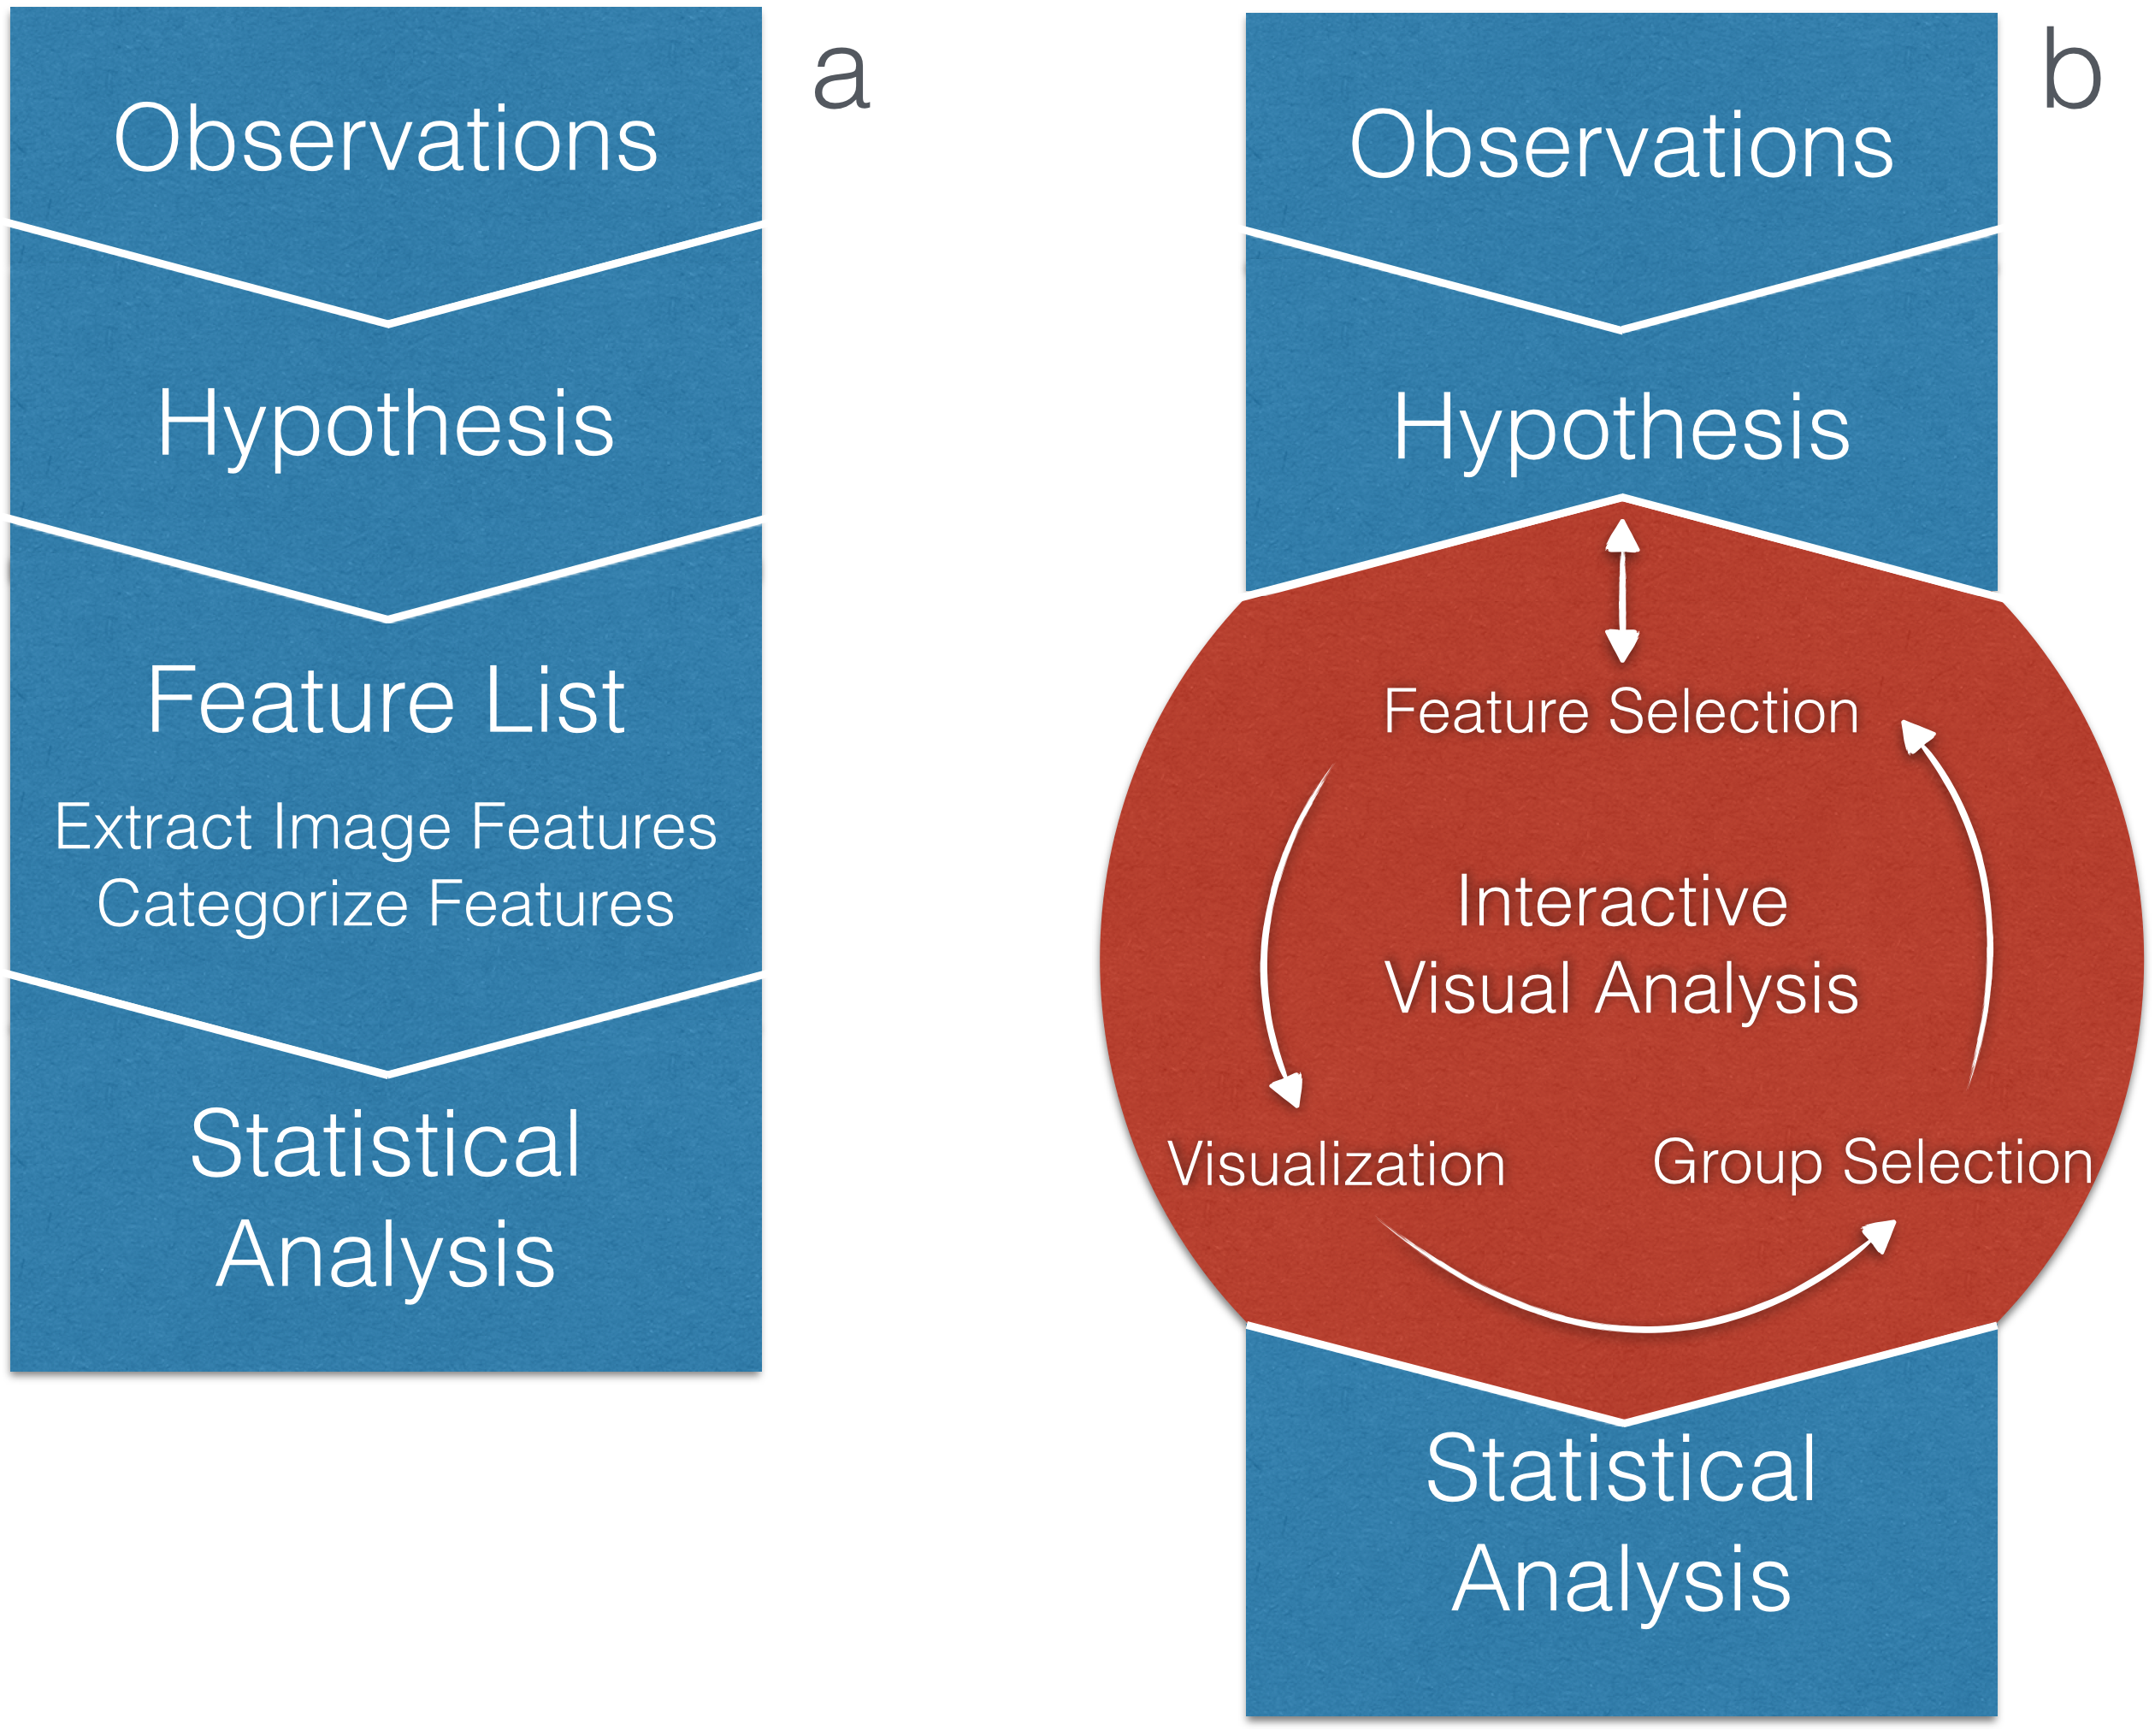
\includegraphics[width=3.0in]{figures/workflow_comparison}
 \caption{ToDo Abbildung noch nicht final. Visual Analytics systems are able to complement parts of the epidemiological workflow, not replace it. The appropriate combination of statistical- and interactive driven analysis shows promising potential to unveil the information in the data. (a) shows the standard epidemiological workflow, (b) the IVA supported one. The iterative red highlighted part is called the \emph{IVA Loop}.}
\end{figure}
- Acceptance plays a big role - you have to pick up the user by presenting information they are used to in a new way\\
%
As described in subsection~\ref{EpidemiologicalWorkflow}, the epidemiolgical workflow is a sequence of steps taken by domain experts and needs to be reproducible and comprise statistical integrity.
%
Figure~\ref{fig:WorkflowComparison} (a) describes this workflow as consecutive series of steps.
%
The workflow we propose by introducing the \emph{IVA} principle into the epidemiological application domain does not aim to replace the existing workflow but to complement its weaknesses.
%
In the current state the workflow treats the data like a black box.
%
A list of features describing the hypothesis is compiled and analyzed using statistical tests. 
%
The resulting value decides whether the data supports the hypothesis or not.
%
It would be possible that there are actually features of the data set which support the hypothesis by discriminating the population in the expected way, but with this approach they are not highlighted in any way.
%
This becomes even more important when the workflow is adapted to the analysis of the medical image data.
%
Domain experts would have to annotate landmarks tediously to derive metrics such as distances. %which are then handled like other features and analyzed using the same set of statistical tools.
%
Not only does this leave out the majority of the information in the medical image data by abstracting it to single values, it is easily possible that information left out would heavily influence the result.
%
Considering more complex parts of the data would make those results more trustworthy and also could identify possible anatomical confounders--an epidemiolgical research result in itself.
%
Statistical tests check for validity of the number but not for their completeness or plausibility!
\\\\
\emph{IVA} tries to illuminate the black box by making the domain experts part of the feature list selection process.
%
Figure~\ref{fig:WorkflowComparison} (b) highlights the iterative process as part of the epidemiolgical workflow.
%
Note that it also aims to project back into the hypothesis formulation step to amplify hypothesis generation 
%
This has to be handled with care since overfitting of expectations to the available data is an imminent danger as described by Turkay and colleagues \cite{Turkay2013}.

\subsection{Image Centric Cohort Study Data in Interactive Visual Analytics Context}
In the \emph{IVA} context, data is divided into two major view types.
%
The human body exposing shape information for the \emph{physical view} \cite{Oeltze2013}.
%
This information space is usually displayed via volume rendering techniques \cite{Oeltze2007}.
%
%Spatiotemporal views include data from the \emph{Object Space Domain} renders data centered to the focused domain, in our example the medical image data space.
%
These variables are also referred to as \emph{independent variables}.
%
\emph{Dependent variables} in the epidemiological context can be divided twofold:
%
\begin{itemize}
	\item Variables derived from the image data. 
	%
	These measures abstracts shape information as quantification to allow for comparison. 
	%
	These variables describe image data and can also be used to brush in the image space.
	\item Epidemiological socio-demographic or medical attribute data.
	%
	These values belong to every subject which is represented in the image space, but does not describe shape information.
	%
	This is the data epidemiologists usually want to correlate with image data.
\end{itemize}
%Other data associated to elements in the object space are considered to be the \emph{Attribute Space Domain} and are displayed using various range based views using statistical graphics and information visualization techniques like scatterplots, bar charts or parallel coordinates \cite{Oeltze2013, Oeltze2007}.
%
%Specific for the epidemiological application domain is that both Object- and Feature Space Domain influence the outcome of interest.
% \textbf{Object Space}\\
% - Medical Image Data / Spine Segmentations\\
% \textbf{Attribute Space}\\
% - SHIP-Variables\\
% - Derived visualizations
% 
% ? Where to incorporate Levels of IVA

\subsection{Data Preprocessing}
To include heterogenous epidemiological data in an \emph{IVA}-framework it is necessary to process it to obtain standardized views to the available features.
%
Multimodal features require different techniques.
%Due to the different acquisition modalities there have to be different techniques incorporated.
%
Data obtained using questionnaires or medical tests are often stored using statistical packages such as \texttt{SPSS} or \texttt{Stata} which have a proprietary data format with limited export capabilities.
%
The best solution for us was to simply export the data in the respective tool to a character separated text file and then convert it to data types which are easier manageable such as JSON or XML using our own classes.
%
In order to verify that the conversion worked as expected and the data is valid, it is good practice to use data wrangling tools such as \texttt{OpenRefine} to validate the data (find missing data, clean up bad formatting).
%
Exporting the data dictionary, which stores information about each manifestation of a feature is also an important step to get a detailed description of data variables and the meaning and unit of measurement of their values.
%
The reasons for missing data have a wide range from ethical to medical and personal issues.
%
Therefore, these are also included as error codes which have to marked as such in the data dictionary.
\\\\
Processing the image data associated to each subject consists for the most part of information extraction about a anatomical structure.
%
This is either done manually by experts setting landmarks (sometimes supported by algorithms connecting the land marks such as graph cuts \cite{GraphCut}) or by a (semi)-automatic detection, registration and segmentation.
%
Algorithms, applied to the data, do not only have to deal with a large inter-subject variability of the anatomical structure, but also need to be reproducible \cite{Preim2014}.
%
Model-based approaches have shown in principle to be effective for segmentation \cite{Gloger2010, Gloger2012} and detection \cite{Rak2013}.
%
If a segmentation yields only binary masks separating the structures, algorithms such as Growing and Adaptive Shapes can be applied creating a surface grid where each point is comparable throughout the population \cite{Ferrarini2007}.
%
Intensity-based comparisons can be achieved using rigid image registration, but model based results however are preferable \cite{Klemm2012}.
%
Comparison based on grey values is usually carried out to to measuring the quantity of fat, water, and--application specific--iron content (liver) or distribution of grey and white brain tissue.

Morphometric variables are derived to allow for statistical comparison of the tissue which incorporate mostly position, volume and relative distances and alignment to other structures.
% 
% - Data Format\\
% - Missing Data\\
% - Registration of Image Data (VMV'12)\\
% - Extraction of Image Parameter

\subsection{IVA Patterns}

The explorative procedures when analyzing data using \emph{IVA} can be divided into three different patterns, handling interaction between domain and range variables.

\subsubsection{Local Investigation}
This pattern projects information from image space to the range perspective.
%
As opposing to other \emph{IVA} application domains, this step is more complicated in the epidemiological context.
%
Shape information can not be brushed by incorporating ROI-selections but rather has to employ techniques that specify local deformation changes \cite{Hermann2014} or subjects that belong to a shape class.
%
Methods available for \emph{feature selection} strongly depend on the type of registration that was applied to extract the tissue of interest.
%
Model-based segmentations or masks yield data structures capable of calculating mean shapes and distances between individuals or subject groups.
%
Feature selection is also possible by applying clustering algorithms in order to get shape-groups \cite{Klemm2013VMV}.
%
These algorithms can be used to investigate interactions between shape-groups and other non-image based variables.
%
Another application is the outlier analysis.
%
Outliers can indicate segmentation errors or an outstanding group of individuals who may share a pathology.

% Local Investigation
% - Projection from Image Space to Attribute data. This is more difficult in our application, because we currently only brush on derived features.\\
% - Clustering in Image Space yields Groups which can be analyzed using the attribute space\\
% - Create a Pipeline Overview over different Levels of different IVA Patterns and Stages

% \subsection{Feature Selection}

% \subsection{Brushing the information space}
% - derive new groups which serve as input for the feature selection

\subsubsection{Feature Localization}
% Subset selection of range variables yields features
As described before, the vast majority of data points are considered to be dependent with respect to the image domain in the \emph{IVA} context.
%
Selecting subjects based on image derived data can be seen as additional possibility of shape-related grouping.
%
The epidemiologist is primarily interested in the shape of subjects within a range of a set of variables that describe the current hypothesis.
%
Epidemiologists are used to categorize data into groups that fit their hypothesis formulation.
%
Continuous variables such as age are for example often divided in categories like young, aged and elderly.
%
Categorization is strongly dependent on the hypothesis and therefore requires suitable brushing techniques as described in Section~\ref{sec:AdaptiveFeatureVisualization}.
%
%To gain insight into interactions between SHIP-

% - Selection of Information using Bar Charts, Scatterplots or Parallel Coordinates which projects the selection into the Object space\\
% - this selection is for categorical data already given implicitly bei projecting the 3D-View onto the Bar Charts/Mosaik Plots!\\
% - this aims to locale features of the data!\\
% - Gain Information about SHIP-Variables by putting them into the context of each other. The Pivot Table allows for direct numerical\\ analysis, while the information visualizations allow for better insight of the combination

\subsubsection{Multivariate Analysis}
%Introduced in the information visualization, the multivariate analysis means selecting subjects in like in the feature localization step and get have the result highlighted in another linked view displaying other non-image parameter.
Introduced in the information visualization, the multivariate analysis incorporates brushing and linking of of views displaying non-image parameter.
%
%This represents for the most part the usual approach which essentially is the analysis of how variables interact with each other, only in a visual analysis context.
%
The need of statistic measures which describe how variables correlate with each other given the selected groups is special for the application domain.
%
These associations also summarized using Pivot Tables which are popular in epidemiology and which are described in the following section.
% - Selection of Elements in Scatterplots, Barcharts or Parallel Coordinates Views - observe how selection changes another view - this allows for multivariate analysis\\
% - Becker, R.A., Cleveland, W.S.: Brushing scatterplots. Technometrics 29(2) (1987)\\
% - Wang Baldonado, M.Q., Woodruff, A., Kuchinsky, A.: Guidelines for using multiple views in information visualization. In: AVI ’00: Proceedings of the working conference on Ad- vanced visual interfaces, pp. 110–119. ACM Press, New York, NY, USA (2000). DOI\\ http://doi.acm.org/10.1145/345513.345271
% - By brushing individual parameters or create new binnings of parameter it is possible to see how they change in coordinated views. This is already implemented in the Cargo framework\\
% - by creating comparative 3d Visualizations it is possible to assess the influence of non-image parameters to the visual space.

\section{Interaction- and Visualization Techniques} \label{Interaction- and Visualization Techniques}
% TODO: Bernhard: Section anders beginnen!
We employ the fourth and highest level which includes next to brushing and linking, advanced brushing, extraction of attributes the development of visualizations custom tailored to the data sets.
\begin{figure}[htb]
 \centering
 %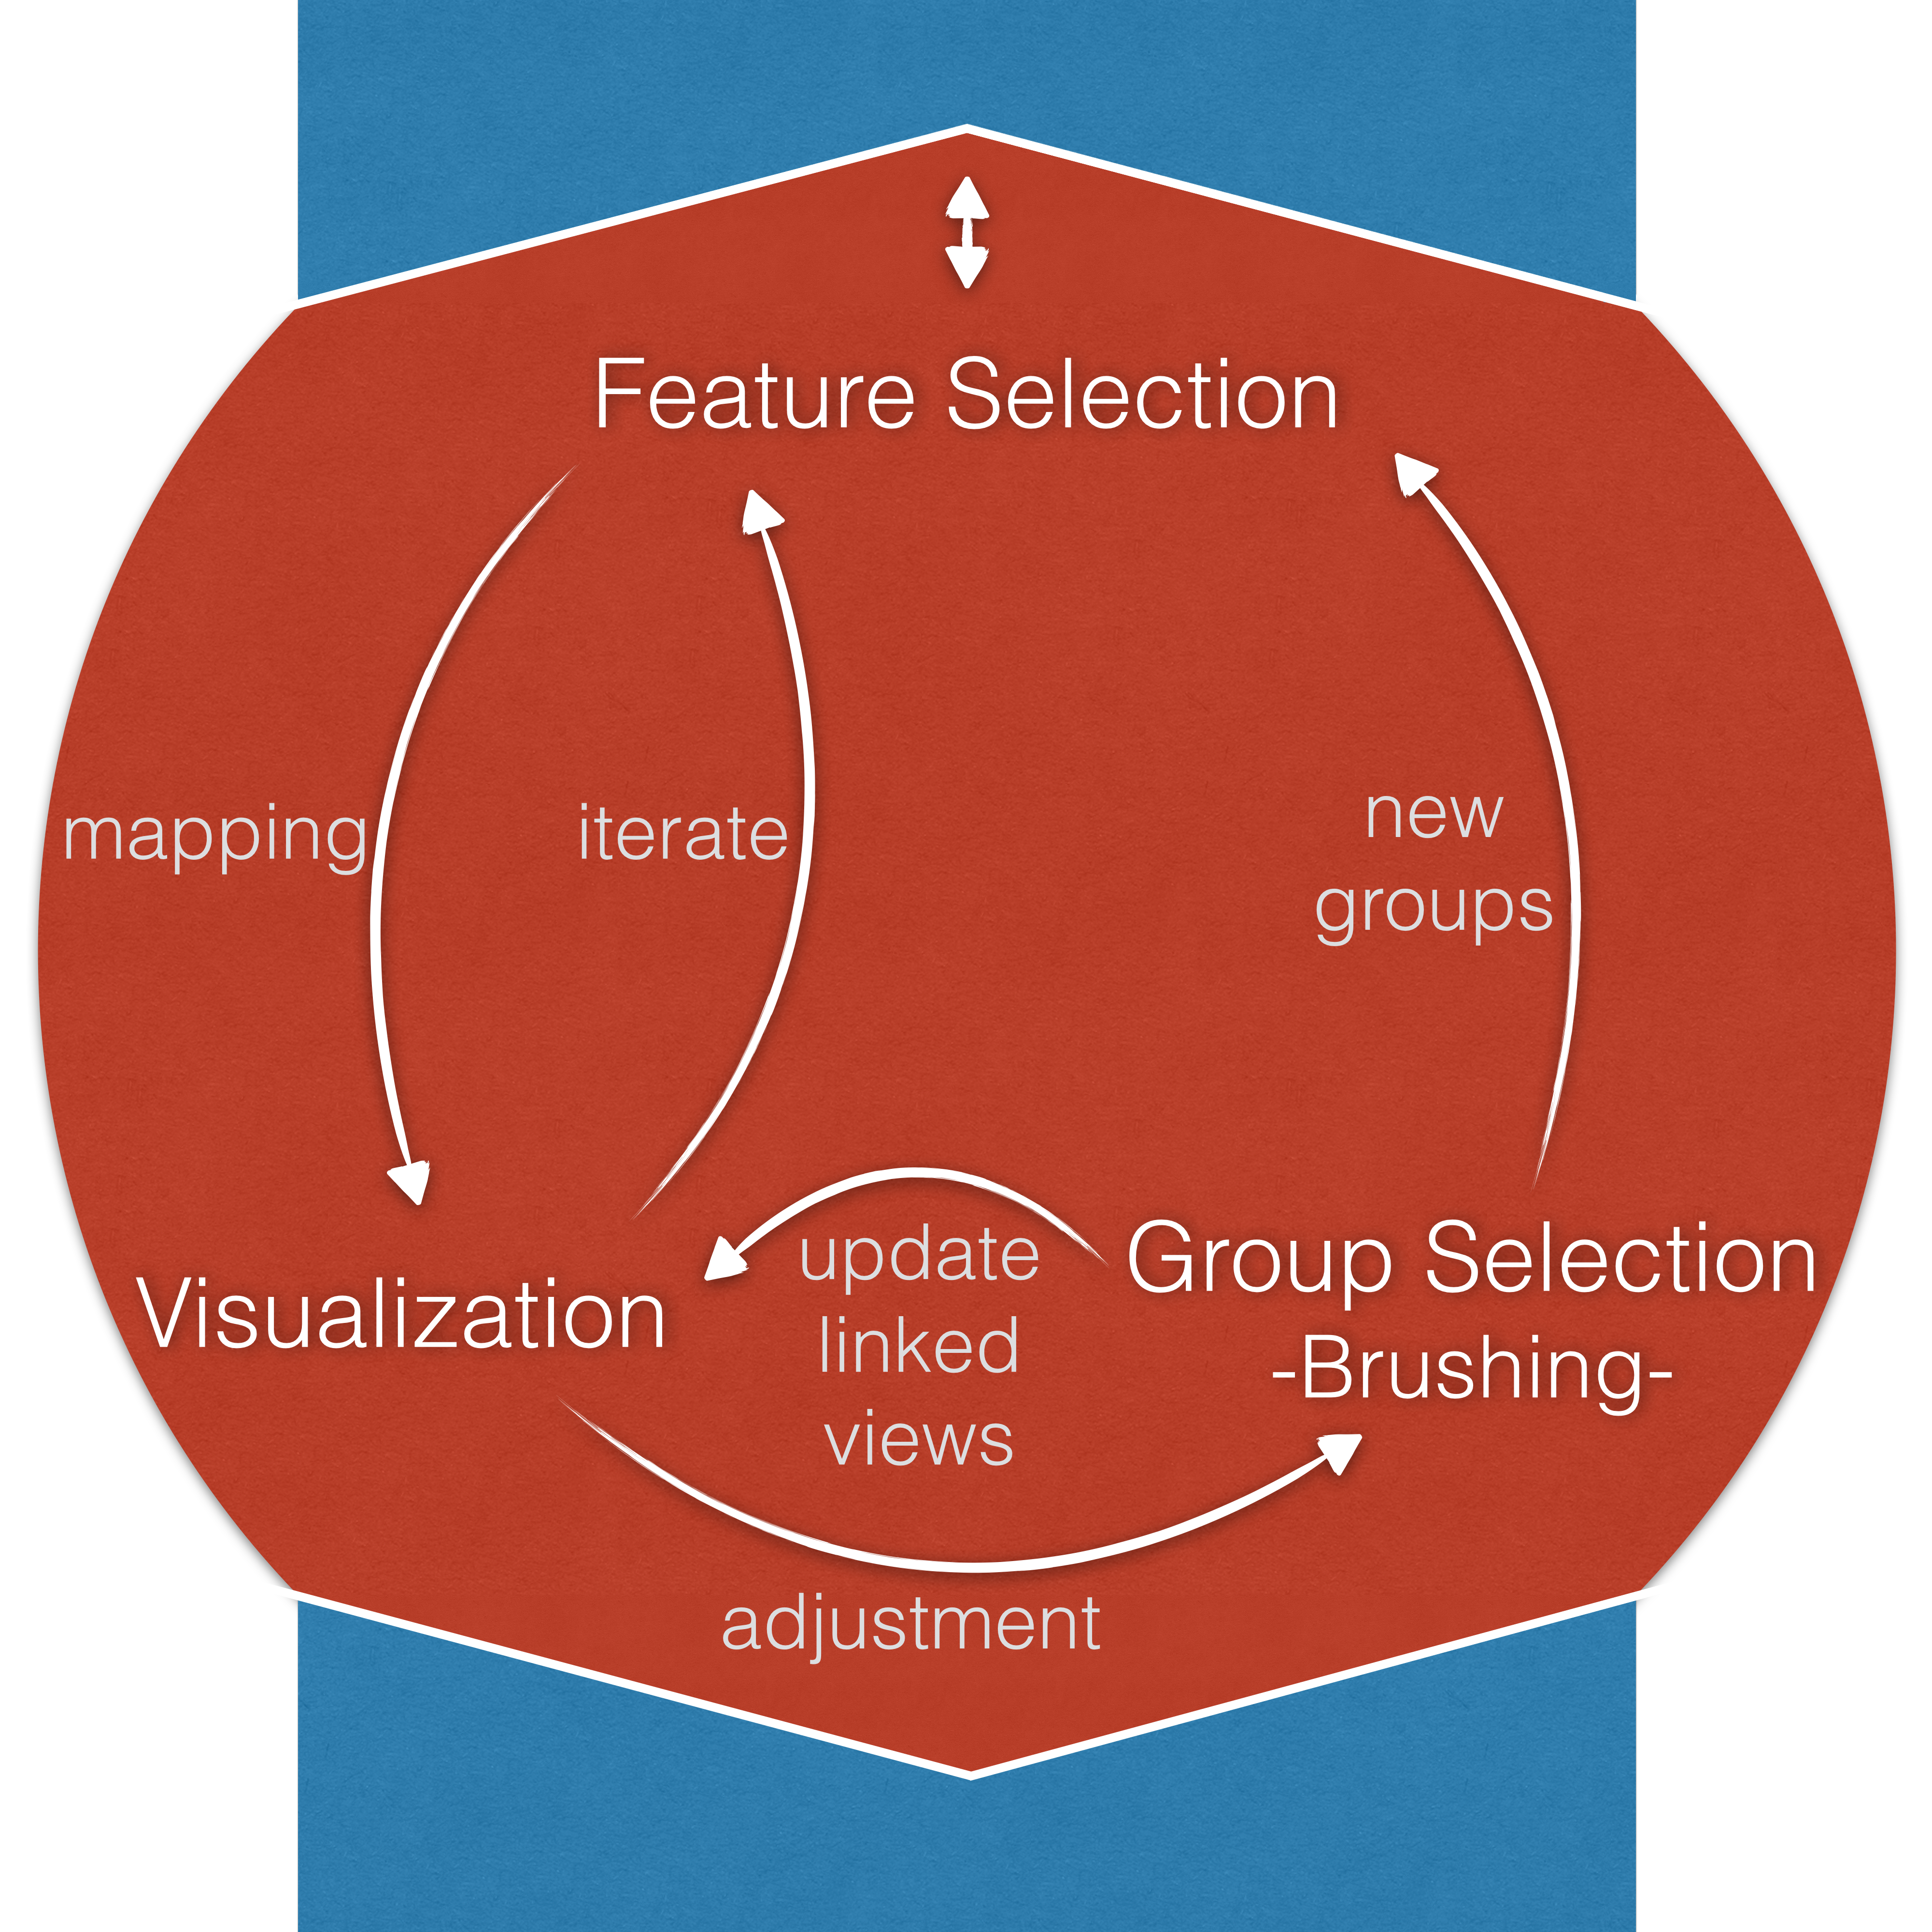
\includegraphics[width=1.5in]{figures/InteractionLoop}
 \includegraphics[width=3.5in]{figures/visualization}
 \caption{\emph{Image is not final} Screenshot from the front-end which is divided as follows: (a) Sidebar which contains all features as well as the groups defined in the analysis process; (b) Canvas area where features can be added via drag and drop and the visualization chosen automatically according to the data type; (c) Interactive Pivot Table which shows exact numbers for each displayed variable combination. The data displayed is used to analyze the lumbar spine.
 }
 \label{fig:visualization}
\end{figure}
\emph{IVA} levels define different levels interaction. 
%
The employed techniques needs to respect the epidemiological requirements.
%
Hypothesis generation bears the chance of over-fitting the data to expectations.
%
To avoid this, a timeline needs to be introduced which keeps track how many variable variations the user evaluated before coming to an conclusion.
%
Since epidemiologists are used to process groups based on table representations we decided to introduce an interactive solution in form of a Pivot Table.

\subsection{Structure and Workflow}
We divide the workspace into three major parts as seen in Figure~\ref{fig:visualization}.
%
\begin{figure}[htb]
 \centering
 \label{fig:InteractionLoop}
 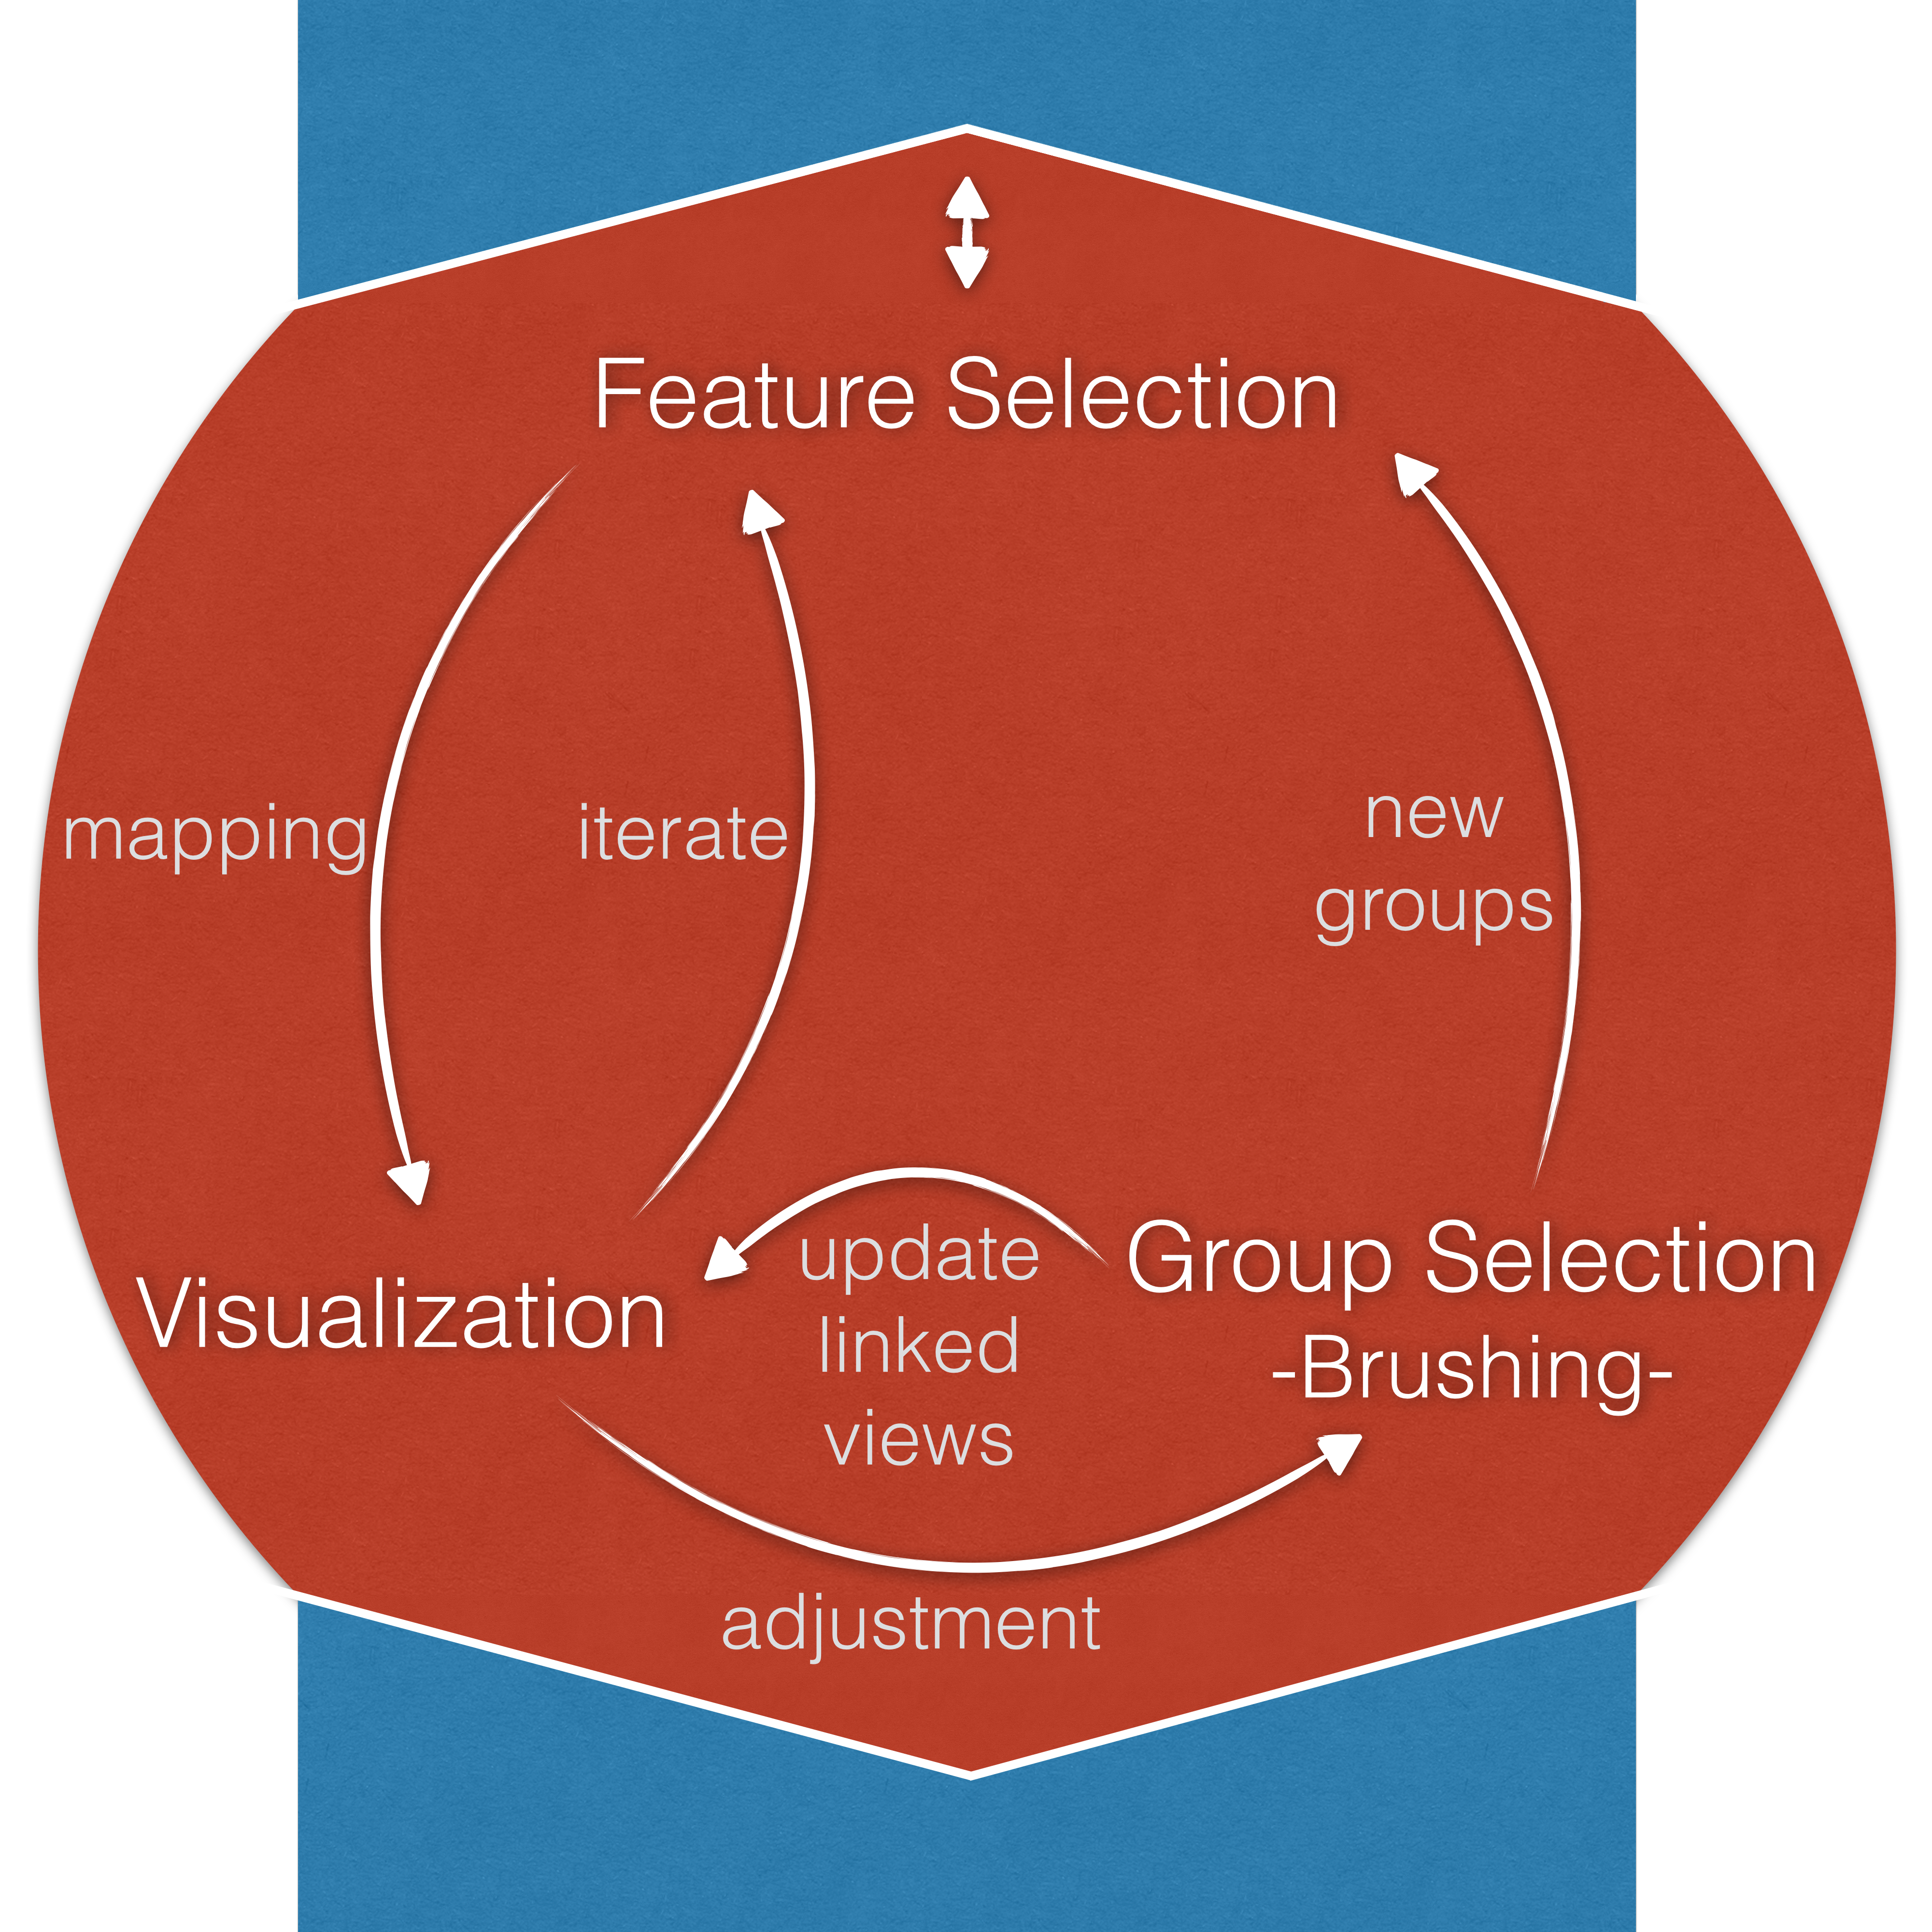
\includegraphics[width=3.0in]{figures/InteractionLoop}
 \caption{Detailed Version of the \emph{IVA Loop}. Usually starting with a selection of Variable of interest (user-driven or via data mining techniques), the data is mapped using a visualization technique appropriate for the selected data types. The data is visualized in the independent and dependent domain space, which can then be brushed, yielding new groups which can be investigated using further variables. Note that adjacent steps are directly connected via feedback loops allowing for iterative refinement and give as much freedom to the user as possible.}
\end{figure}
TODO auf Fig~\ref{fig:InteractionLoop} zurückkommen
%
The sidebar holds all available variables as well as groups either derived by user input or automatic clustering.

From the sidebar, elements of interest can be put into the canvas area via drag and drop.
%
Doing so will automatically create an information visualization suitable for the current data type.
%
3D shape information about the investigated structure is displayed for each variable manifestation.
%
By dropping variables on existing visualizations the system creates a visualization that allows for comparison (e.g. mosaic plots for ordinal variables).
%
Elements can be brushed in the information visualizations and are linked to the other representations in the canvas.
%
Shape based clustering can either be applied to all subjects or subgroups.

All elements in the canvas view are also represented in the interactive Pivot Table which gives detailed information how the subjects are distributed given the displayed variables.
%
Details to the different views are presented in the following sub-sections.

ToDo\\
- wie werden Confounder gefunden?\\
- welche statistischen Kennzahlen werden eingebunden?\\

\subsection{Sidebar}
An overview of all variables is presented in a sidebar where they are categorized to different types such as somatometric, disease- or lifestyle related, pain indicators and laboratory data.
%
It also contains subject groups either defined by user brushing or by automated clustering.
%
Groups are treated exactly like other variables since they work exactly the same way which is dividing the subject space into different labeled categories.
% TODO Implement
Bar charts show the distribution of manifestations of each variable in the sidebar.

\subsection{Adaptive Feature Visualization} \label{sec:AdaptiveFeatureVisualization}
Inspired be the previously discussed \emph{GPloms} \cite{Francois2013} the visualization type is chosen dynamically based on the variable types and number of visualizations which need to be displayed.
% TODO Implement MOSAIC PLOTS, Scatterplots, Parallel Coordinates
If possible the medical image data is directly included into the plot as well by including mean shapes for each manifestation (Figure~\ref{fig:visualization} (b)).
%
The 3D-plots can be navigated using standard mouse inputs and the camera is synchronized so that a direct comparison is given.
%
If a feature is dropped on an existing plot, the visualization changes dynamically to properly make them comparable. 
%
Each plot can be brushed using widgets.
%
It is able to duplicate brushes in order to create new groups which are evenly spread out.
%
A use case for this is when a continuous feature has to be divided into even groups.
\\
ToDo\\
- Dichotomous data\\
- Time-Line\\
- Statistical Analysis (Odds ratios)\\

TODO 2\\
- 3D Plots are small multiples - reference Tufte!

\subsection{Pivot Tables}
Pivot tables are frequently used to present the data in epidemiological paper.
%When opening a random epidemiological paper the reader will in almost all cases find some sort of pivot table to present the data.
%
As seen in Figure~\ref{fig:visualization} (c) it is a good way to display how many subjects are in each group.
%
Pivot table quickly get confusing and cluttered when they are divided into to many subgroups.
%
We tackled this problem by making the order and number of displayed variables adaptable.
%
This also applies on the designation of Row or Column Variables.
% TODO IMPLEMENT
The mean shape for each resulting sub-group is also displayed for each subject.

\subsection{Automated Feature Suggestion}
% https://de.wikipedia.org/wiki/Kontingenzkoeffizient#Cram.C3.A9rs_V
TODO REWRITE USING CRAMERS V

As discussed previously, highlighting potential interesting values in the data set is one major benefit of the \emph{IVA} powered approach.
%
Turkay and colleagues used the approach to calculate various key figures based in the distribution functions of each feature derived from the image data \cite{Turkay2013}.
%
Since the majority of our data are categorical features, we have to employ different solutions.
%
A solution for this problem are odds ratios, which are a standard statistical tool for stating relations between features.
%
Odds ratios can only be calculated for $2\times2$ contingency tables which usually represent the presence of a condition in a population divided by a characteristic (e.g. male/female subjects with presence or absence of back pain).
%
To calculate odds ratios for variables with more than two manifestations, we calculate local odds ratios for each possible combination, yielding a matrix for each feature combination \cite{Rudas1998}.
%
When the subjects are divided into groups and the calculation is carried out again for all feature combination, the difference in sum of the odds weighted with the number of manifestations per feature can be used to indicate if the feature combination yields a difference.
%
These difference are then highlighted in a separate tab of the side bar "Interactions".
%
Interesting interactions then can be assessed creating a linked view using the standard drag and drop workflow.
\\\\
In the following sections we will discuss details on the implementation which relies on modern Web-Technologies.
\\\\
ToDo\\
- This can be improved--summing up the values possibly not the cleverest solution--calculation of variance etc. possible\\
- Matrix Visualization?



\subsection{Implementation}
\begin{figure}[htb]
 \centering
 \label{fig:technologies}
 %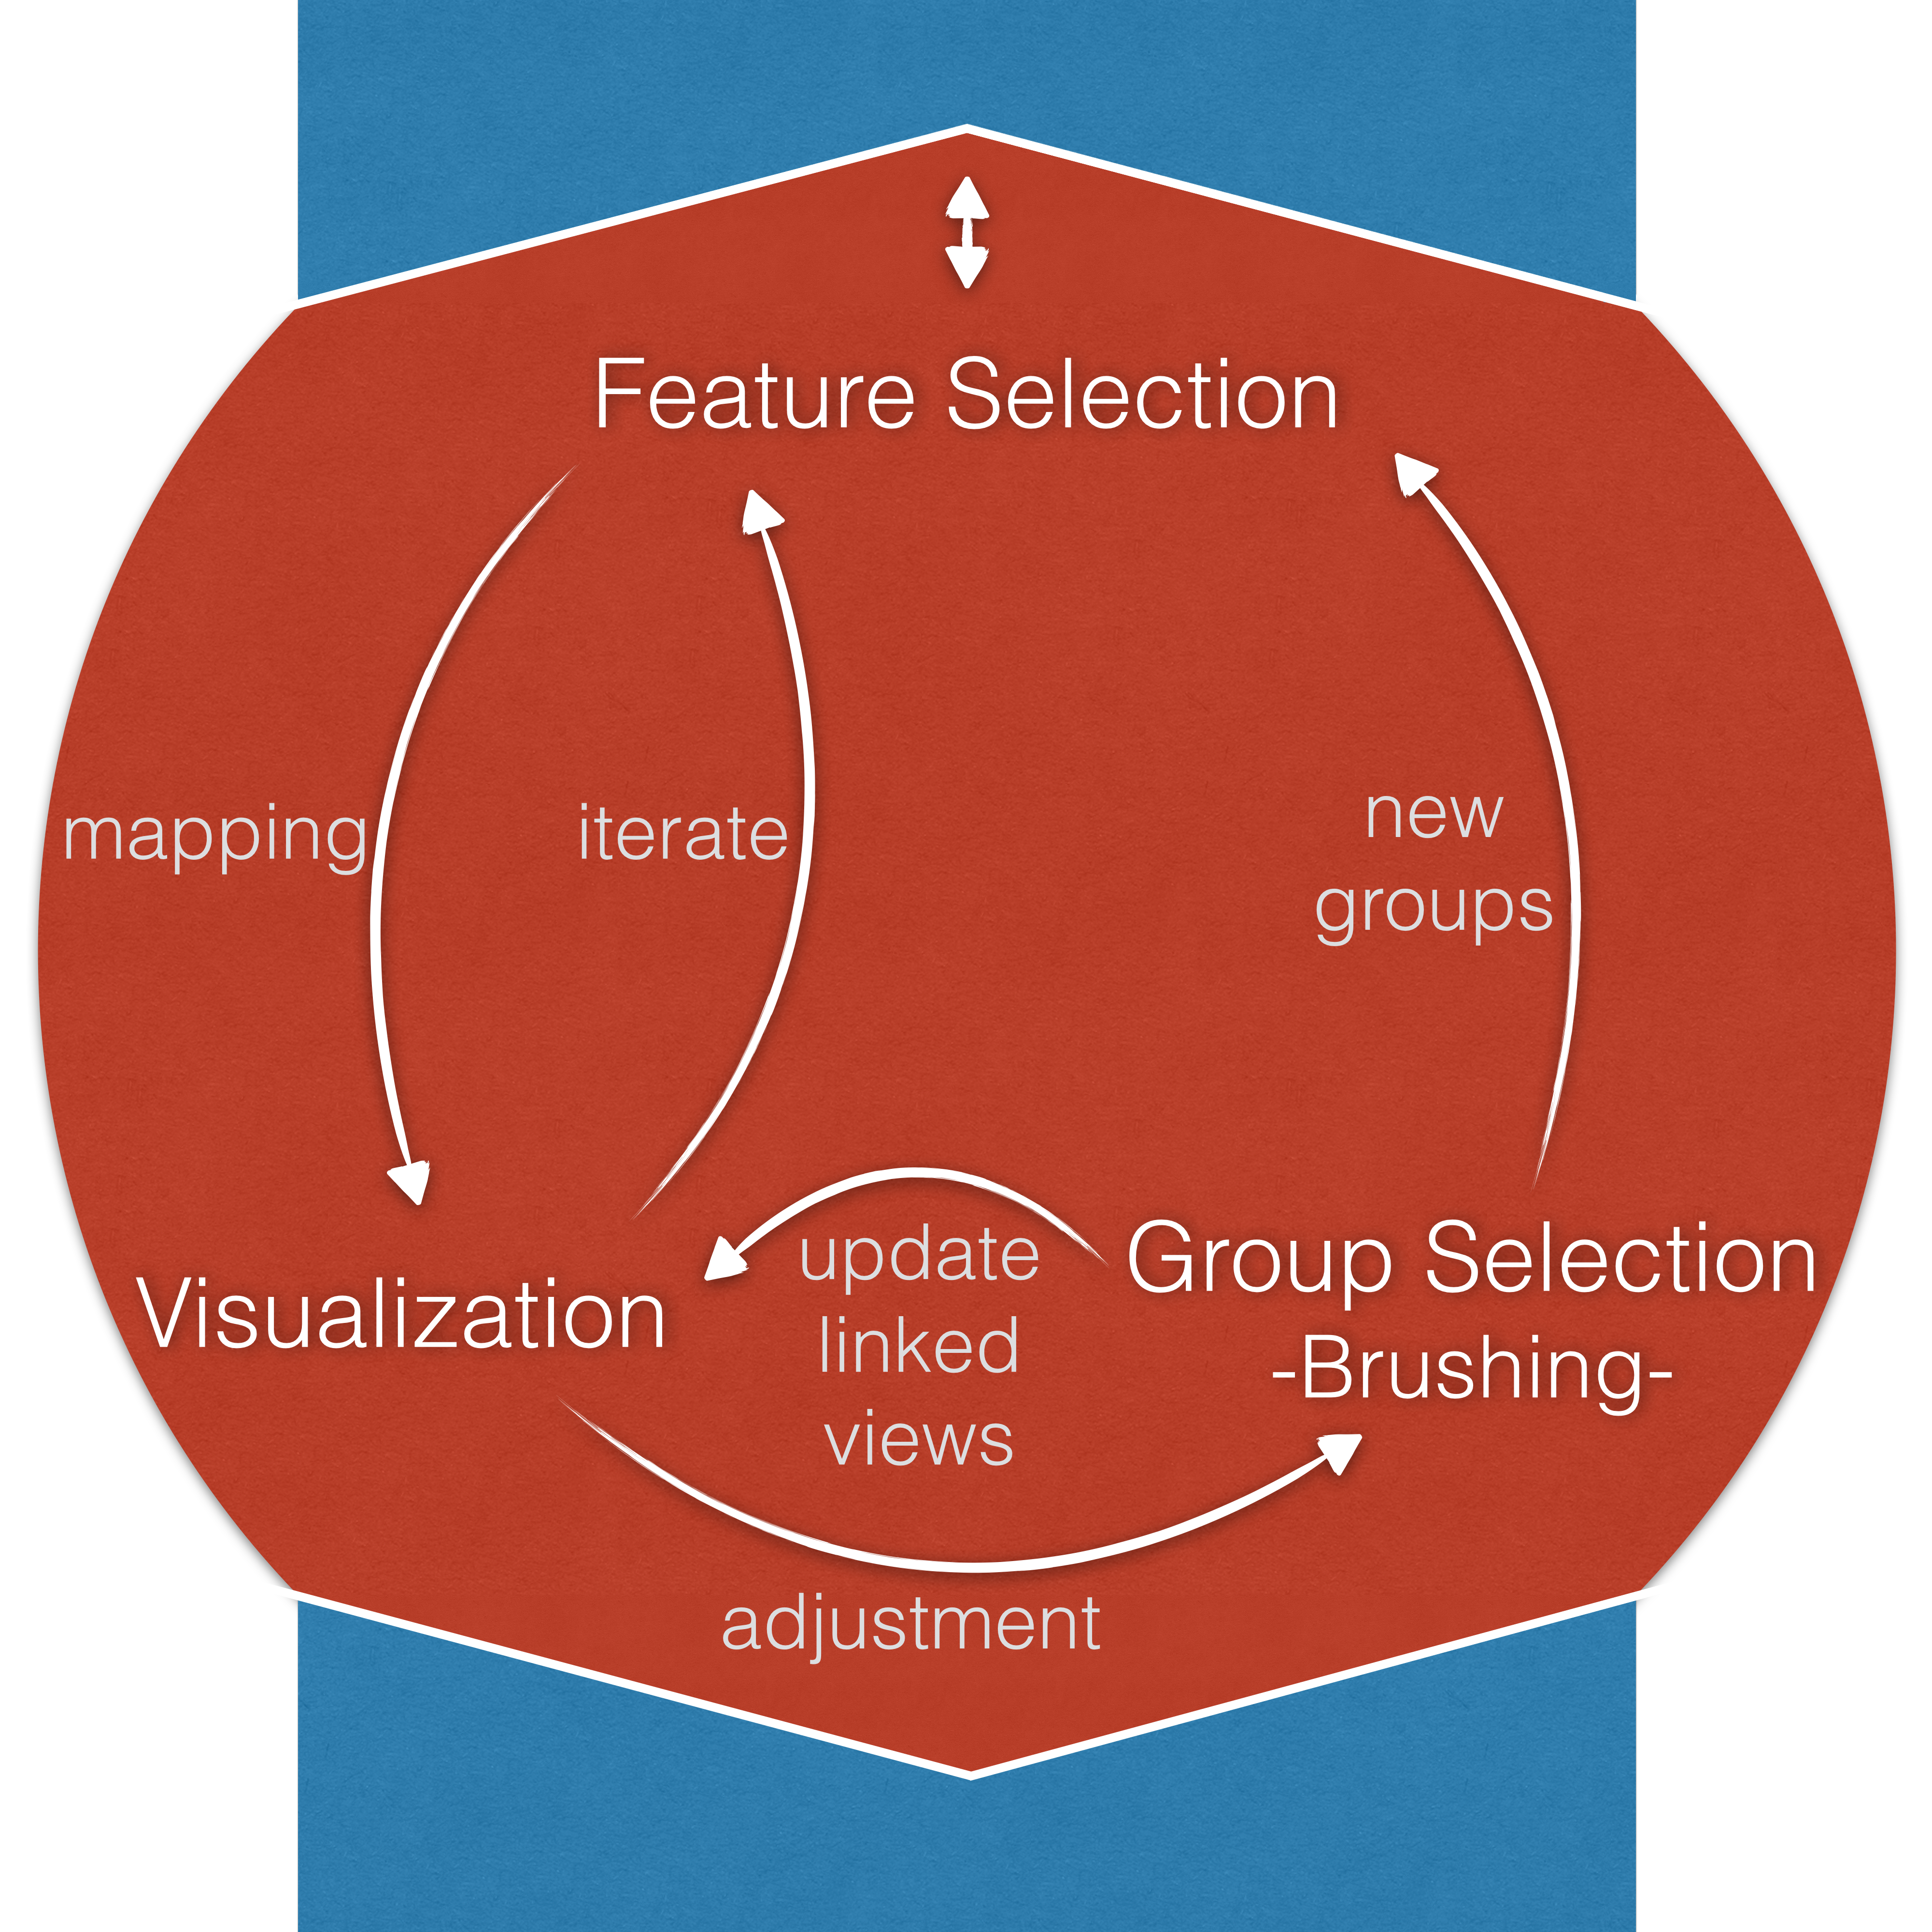
\includegraphics[width=1.5in]{figures/InteractionLoop}
 \includegraphics[width=3.5in]{figures/technologies}
 \caption{\emph{Image is not final}. The front-end solution (left) uses state of the art web technologies such as HTML5/CSS3, WebGL and SVG to display the data.
 % 
 The NodeJS based back-end (right) stores all image- and non-image data and transfers it to connected clients.
 %
 All computation heavy operations like calculation of mean-shapes or -distances as well as statistical processing is done by the server to keep hardware requirements of client systems low. 
 %
 Client-Server communication is accomplished via the WebSocket protocol.
 }
\end{figure}
%
In order to provide a fast communication loop between method development and expert input, we decided to base all implementations on modern web technologies which benefits from various advantages:
\begin{itemize}
	\item No additional software needs to be installed, most people use decent state-of-the-art web browser, even on mobile devices.
	\item The Client-Server structure allows it to employ heavy computation on a server machine and transfer results to the client
	\item Since image data for several thousand subjects claims hundreds of Gigabytes disk space it can remain safely on the server and elements can be transferred on demand.
	%
	High confidentiality standards of the data can be met by restricting access via a account system
	\item Recent developments in WebGL applications running in browsers with near native performance push the development into to the web which results in many open source libraries which are well documented, rich in examples and driven by active communities.
\end{itemize}
These advantages do not come without drawbacks.
%
Many methods which specialized libraries like the Visualization Toolkit (VTK) or R for statistics have build in need to be written from scratch in order to fit in the context.
%

The back-end is written using Node, which based on the Google V8 Javascript runtime environment.
%
Due to its event-driven non-blocking I/O model it is fast and does not freeze in case of heavy workload like mesh calculation.
\\\\
Non-image data for all subjects including the data dictionary is stored on the Server in a JSON file.
%
Image data is available as raw DICOM files as well as segmented Meshes which can be used to compare subjects.
%
On client connection the requested files are transferred.
%
The server processes calculation heavy statistical tasks such as calculation of Odds Ratios or Chi Square tests for all variable combinations in order to keep the computation time on the client as low as possible.
%

The front-end is created using Twitter Bootstrap as foundation for the layout and basic UI elements using HTML5, CSS3 and Javascript.
%
Information Visualizations such as Scatterplots and bar charts are created using the popular Data Driven Documents library which works well for attaching data to visible elements like vector graphics.
%
WebGL rendering is done using the Threejs which allows GPU Accelerated data rendering.
%
Communication between Client and Server runs through the WebSockets protocol.
%
Since our clustering algorithms are written in MatLab we hat to access them using the Node Server.
%
We accomplished this by converting them to parameterized standalone console applications which are spawned by node on client request and then reads the result from the console standard-out and returns it in a proper format to the client.
%
All parameter steered console applications can be incorporated in this context.

\section{Application}
We applied the presented set of techniques to a data set which is compiled to analyze lower back pain. 
%
It is one of the most common reasons for an adult to see a physicians in the western civilization \cite{Backpain}.
%
Epidemiological analysis of lumbar back pain such the work of Harreby and colleagues \cite{Harreby1996} is largely focused on non-image information.
%
If at all, only a few shape related features are included in comparable studies, for example by Lang and colleagues \cite{Lang2011}.
%
To our knowledge, this is the first approach on analyzing shape related information of the whole lumbar spine with other epidemiological features.
%
Determining risk factors in this area can lead to \cite{Fletcher2012} (evtl. weglassen, Dopplung bei Epidemiological Background?):
\begin{itemize}
	\item a better understanding of effects of preventive measures such as occupational health and safety regulations
	\item prognostic features for diagnosis and treatment of lumbar back pain
	\item determination of particularly effected risk groups
\end{itemize}
% Determining risk factors in this area can lead to \cite{Fletcher2012} (evtl. weglassen, Dopplung bei Epidemiological Background?):
% \begin{itemize}
% 	\item a better understanding of effects of preventive measures such as occupational health and safety regulations
% 	\item prognostic features for diagnosis and treatment of lumbar back pain
% 	\item determination of particularly effected risk groups
% \end{itemize}
%
Characterizing the healthy aging process of the spine is a large stretch goal that allows to determine age-normalized probabilities for spine-related diseases by incorporating individual risk factors.

Data confidentiality and ethical reasons prohibit us from accessing the complete data space of the SHIP feature space.
%
Our clinical partners compiled a feature list which is a tradeoff between complexity and limitations of the responsible ethics committee. (vllt. etwas hart formuliert).
%
%The goal is to find features which \emph{interact} with lower back pain based on image and non-image data.
%
\subsection{The Lumbar Spine Dataset}
We divide the data set in image and non-image data.
%
There are 136 features describing diagnosed diseases, lifestyle factors, women specific factors, pain indicators, laboratory values, somatometric variables and are ordered accordingly.
%
The image data was acquired on a 1.5~Tesla scanner (Magnetom Avanto; Siemens Medical Solutions, Erlangen, Germany) by four trained technicians in a standardized way.
%
The spine protocol consisted of a sagittal T1-weighted turbo-spin-echo sequence (676 / 12 [repetition time msec / echo time msec]; 150$^\circ$ flip angle; 500~mm field of view; $1.1\times1.1\times4.0~mm$ voxels) and a sagittal T2-weighted turbo-spin-echo sequence (3760 / 106 [repetition time msec / echo time msec]; 180$^\circ$ flip angle; 500~mm field of view; $1.1\times1.1\times4.0~mm$ voxels) \cite{Hegenscheid2013}.

\subsection{Data Preprocessing} \label{Data Preprocessing}
Transformation operations on the data to prepare it for the presented prototype are denoted as data preprocessing.
%We denote all data transformation steps necessary outside of our prototype for it to be prepared to work in our prototype as data preprocessing.
%
\paragraph{Image-Data.} \label{Image-Data}
The lumbar spine was detected in the image data using a hierarchical finite element method according to Rak and colleagues \cite{Rak2013}.
%
This semi-automatic method requires the user to initialize the Tetrahedron-based finite element models (FEM) with a click on the L3-vertebra.
%
Two user defined landmarks on the top and bottom of the L3-vertebra are used to obtain an initial height estimation of the model.
%Two more user- defined landmarks are the top and bottom of the L3-vertebra, which transforms size of the model accordingly to match the L3-vertebra .
%
It uses a weighted sum of T1- and T2-weighted MRI images to detect the lumbar spine shape.
%
The registered models capture resilient information about shape of the lumbar spine canal as well as the position of the L1-L5 vertebrae \cite{Klemm2013VMV}.
%
Due to TODO ANTWORT VON MARKO HIER, 983 models are obtained.
%
For clustering purposes we extracted the centerline of the spine canal of the lumbar spine canal which captures information about lordosis and scoliosis which are medical terms for spine curvature \cite{Klemm2013VMV}.

\paragraph{Non-Image Data.} 

To ensure fast and easy data access outside of statistical processors like \texttt{SPSS} or \texttt{STATA}, the data was exported to the JSON file format which can easily be parsed by modern programming languages.
%
Each feature is stored as object which contains: 
\begin{itemize}
	\item the data as array of values--categorical values and error codes are stored using IDs
	\item the data type (continuous, nominal, ordinal, dichotomous)
	\item a detailed description of the variable
	\item the data dictionary which translates value- or error IDs to the actual values
\end{itemize}
%
% Binning: https://www.researchgate.net/post/What_metric_best_captures_the_information_loss_when_binning_a_large_data-set_into_a_histogram_representation
Continuous variables are discretized to allow for \emph{Cram\'{e}rs' V} contingency coefficient assessment.
%
In epidemiology, continuous data is usually categorized into ordinal groups of equal size.
%
Since the number of categories often strongly depends on the hypothesis, the discretization steps can be adapted dynamically.
%
To allow for hypothesis generation we set the number of groups to five if not specified otherwise.
% TODO MIT KAI FORMEL ERARBEITEN?

\subsection{Shape Visualization and Clustering}
%The detection algorithm described in Section~\ref{Data Preprocessing} yields a model that determines voxel belonging to the lumbar spine.
%
The tetrahedron-based model detection model described in Section~\ref{Data Preprocessing} consists of corresponding grid points for each structure instance.
%
This allows for calculation of shape-distance and similarity.
%
This information is used to calculate mean-shapes as described in Section~\ref{Interaction- and Visualization Techniques}.

Shape distance is mapped onto color.
%
For dichotomous variables, the color codes distances between mean shapes of the two groups, for variables with more than two manifestation it encodes the distance to the global mean shape of all subjects (Figure~\ref{fig:hypothesisfree}).
\\\\
Shape based clustering is carried out via Agglomerative Hierarchical clustering of the spine canal ,centerlines which are described in Section~\ref{Data Preprocessing} \cite{Klemm2013VMV}.
%
Since it is not possible to determine the number of clusters in a given group, it is automatically computed using a \emph{knee/elbow} point which is described as tradeoff between number of cluster and a cluster evaluation metric \cite{Salvador2004}.
%
For details, see \cite{Klemm2013VMV}.
%
The method has proven to produce comprehensible results on a preliminary data set and was able to reproduce textbook knowledge \cite{Klemm2013VMV}.

\subsection{Exploratory Analysis of the Lumbar Spine Dataset}
%
%We analyzed the given dataset expert guided to assess its suitability for supporting both hypothesis-free analysis as well as generation.
Expert guided analysis assessed the suitability of our approach for supporting both hypothesis-free analysis as well as hypothesis generation.
%
\subsubsection{Hypothesis free Analysis} \label{Hypothesis free Analysis}
\begin{figure}[htb]
 \centering
 %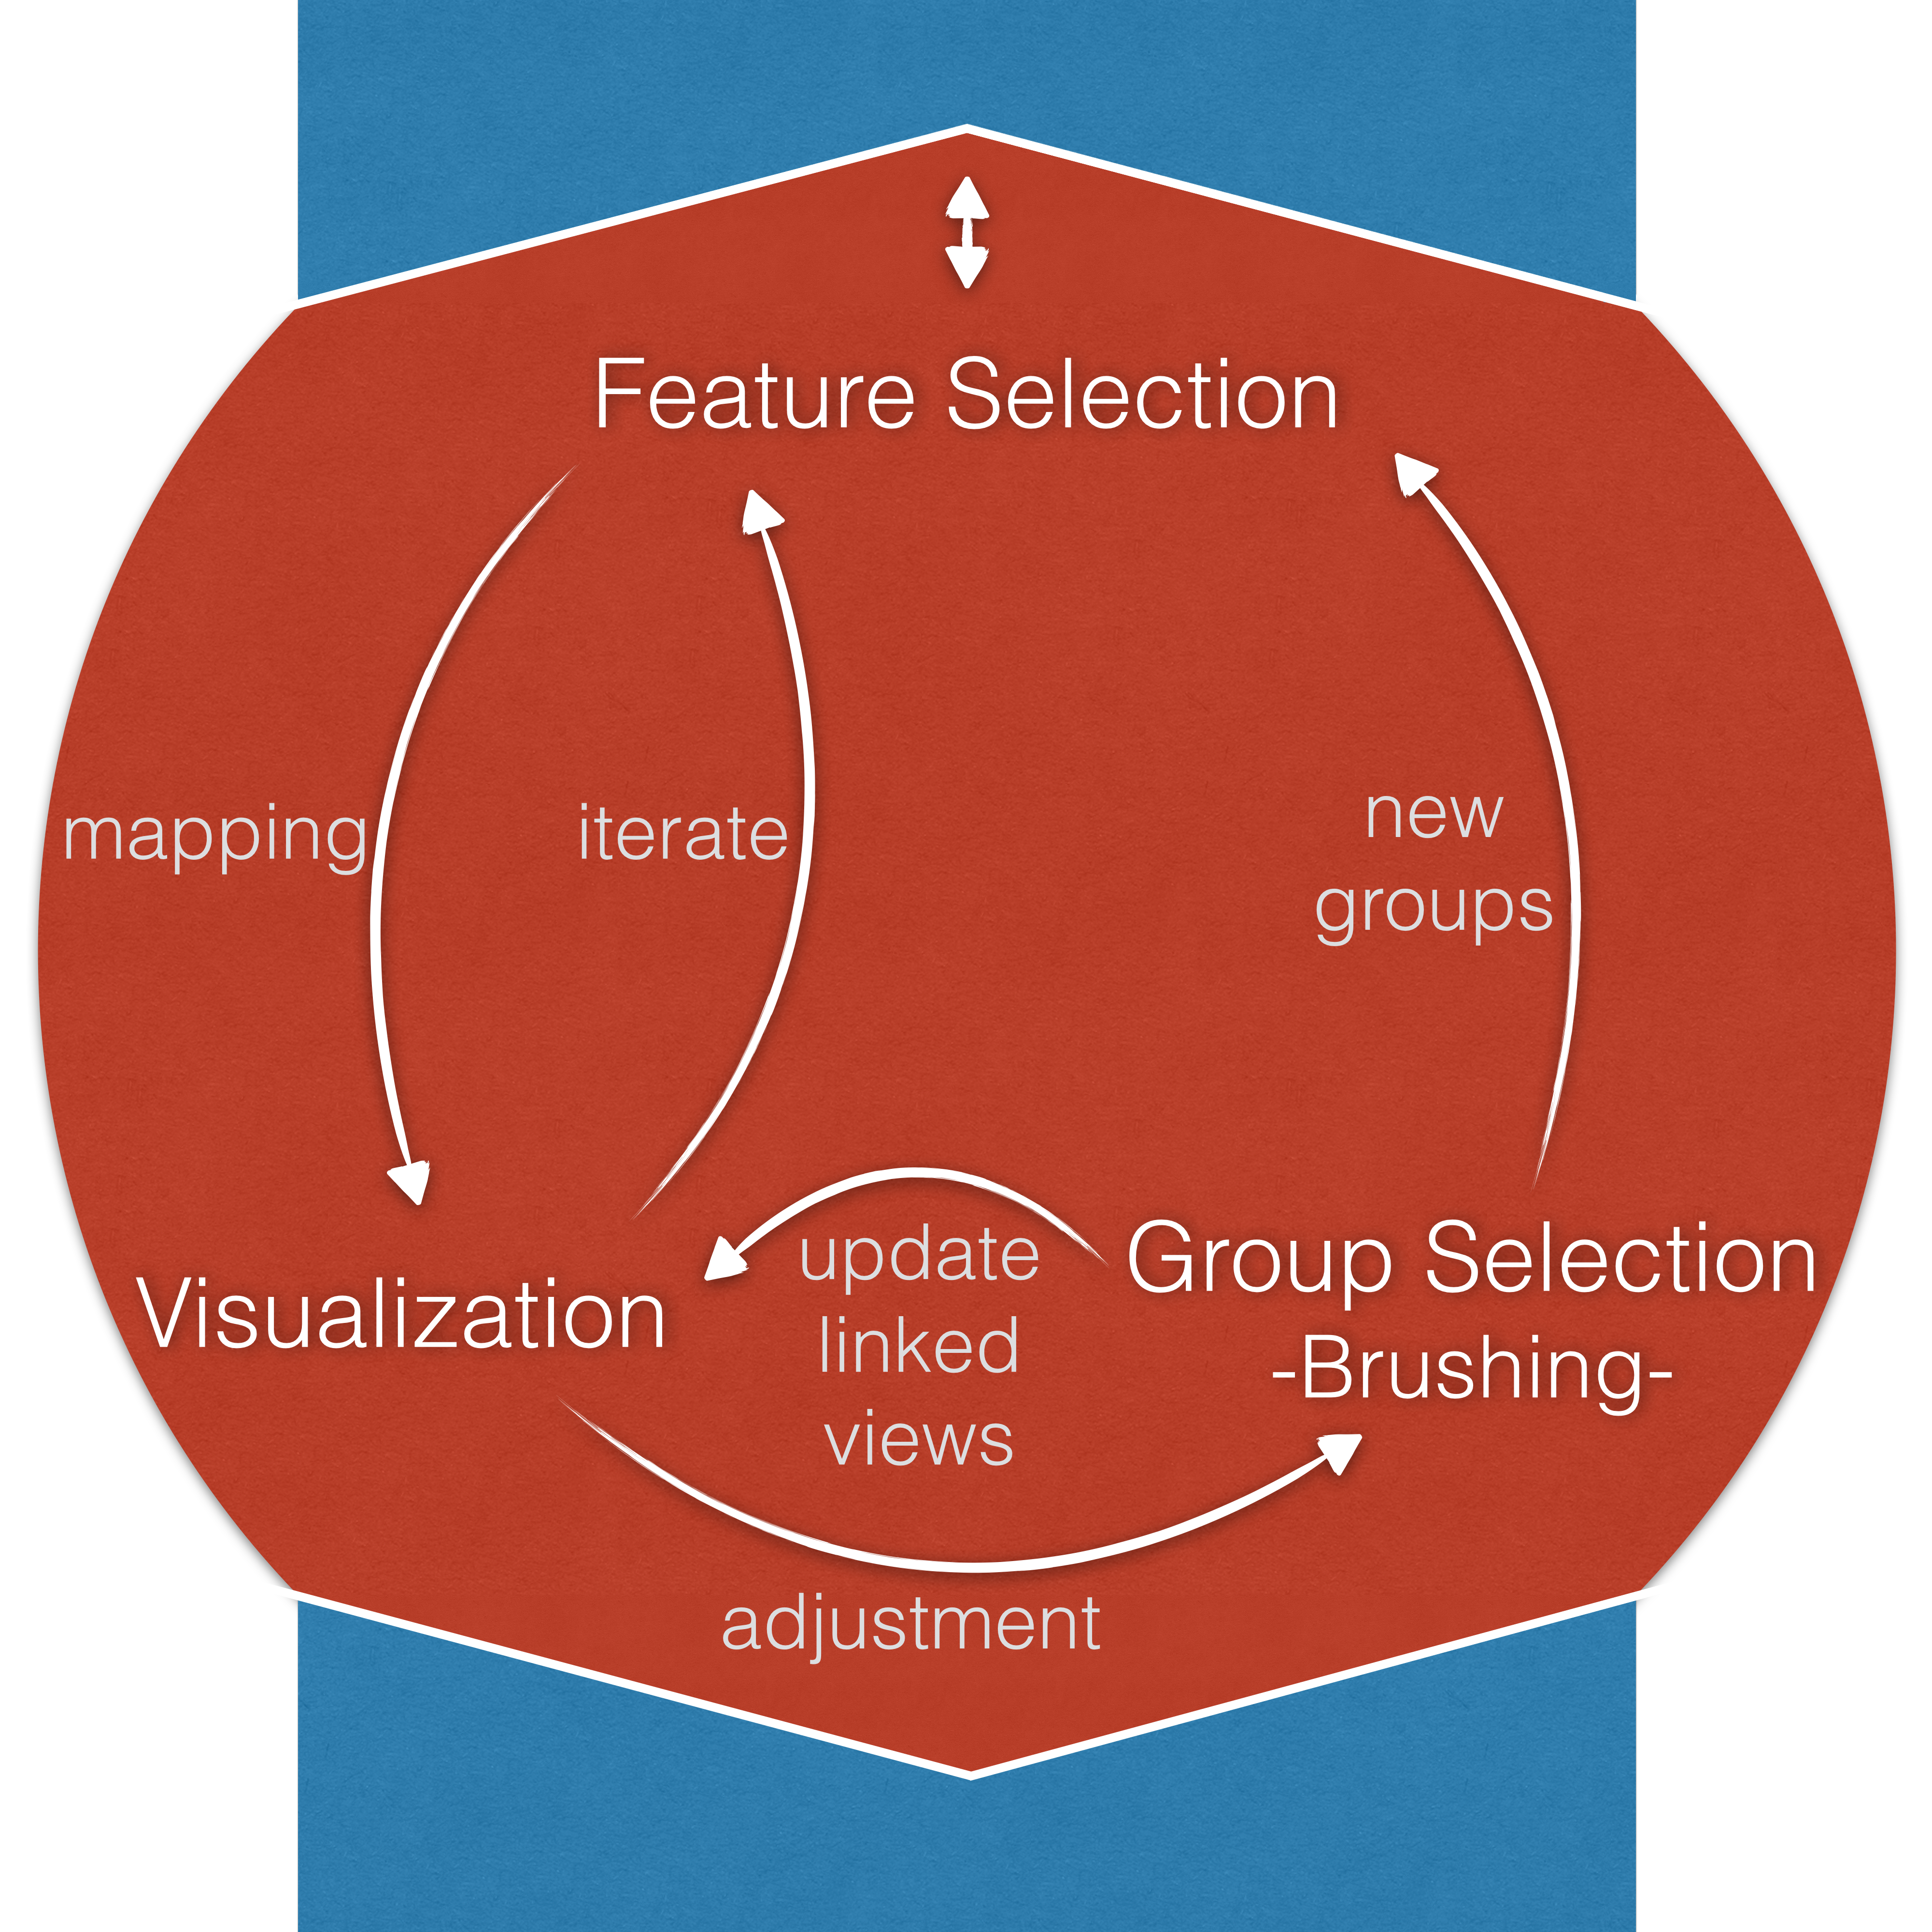
\includegraphics[width=1.5in]{figures/InteractionLoop}
 \includegraphics[width=3.5in]{figures/hypothesisfree}
 \caption{\emph{Image is not final}. (a) Clustering result of all subjects. The bar chart height indicates the number of subjects in the cluster. The difference to the mean-shape is color-coded where blue represents no difference and red a large difference.}
 \label{fig:hypothesisfree}
\end{figure}
%
Analyzing the data set without a prior hypothesis requires a starting point which gives a overview over the data first \cite{Shneiderman1996}.
%
Shape based hypothesis free exploration starts with a shape-grouping step achieved by image-based clustering.
%
The results for this step can be seen in Figure~\ref{fig:hypothesisfree} (a).

Cluster 9 represents the subjects with average shape.
%
Other shapes differ with respect to size, such as Cluster 2, 8, 10 and 3 where the last one also is more straight, which is usual for subjects with larger body height.
%
Cluster 4, 7 and 5 contain outliers, characterized by their unusual shape and small number.
%
Cluster 8 was of special interest because of its large distance to the mean shape while still exposing the second highest subject count.
%
Looking at the \emph{Cram\'{e}rs' V} contingency values of the group reveals interactions of this group with employment status, body size, age, thyroid nodules and blood-fat value.
%
TODO Feedback einholen von Frau Hegenscheid, TODO Implement Color coding only in a certain direction!\\
TODO Selection of the variables and display them using the pivot table!
\\\\
While this approach does not assume any hypothesis, the data is met with a selection bias when compiling the list of related features by the domain experts.
%
It is arguable if this first filtering step, which is purely based on expert experience, is really a disadvantage, since it rules out many parameters which may interact with the presented features but the value of this knowledge would be small \cite{Wiley2008}.

\subsubsection{Hypothesis based Analysis} \label{Hypothesis based Analysis}
\begin{figure}[htb]
 \centering
 %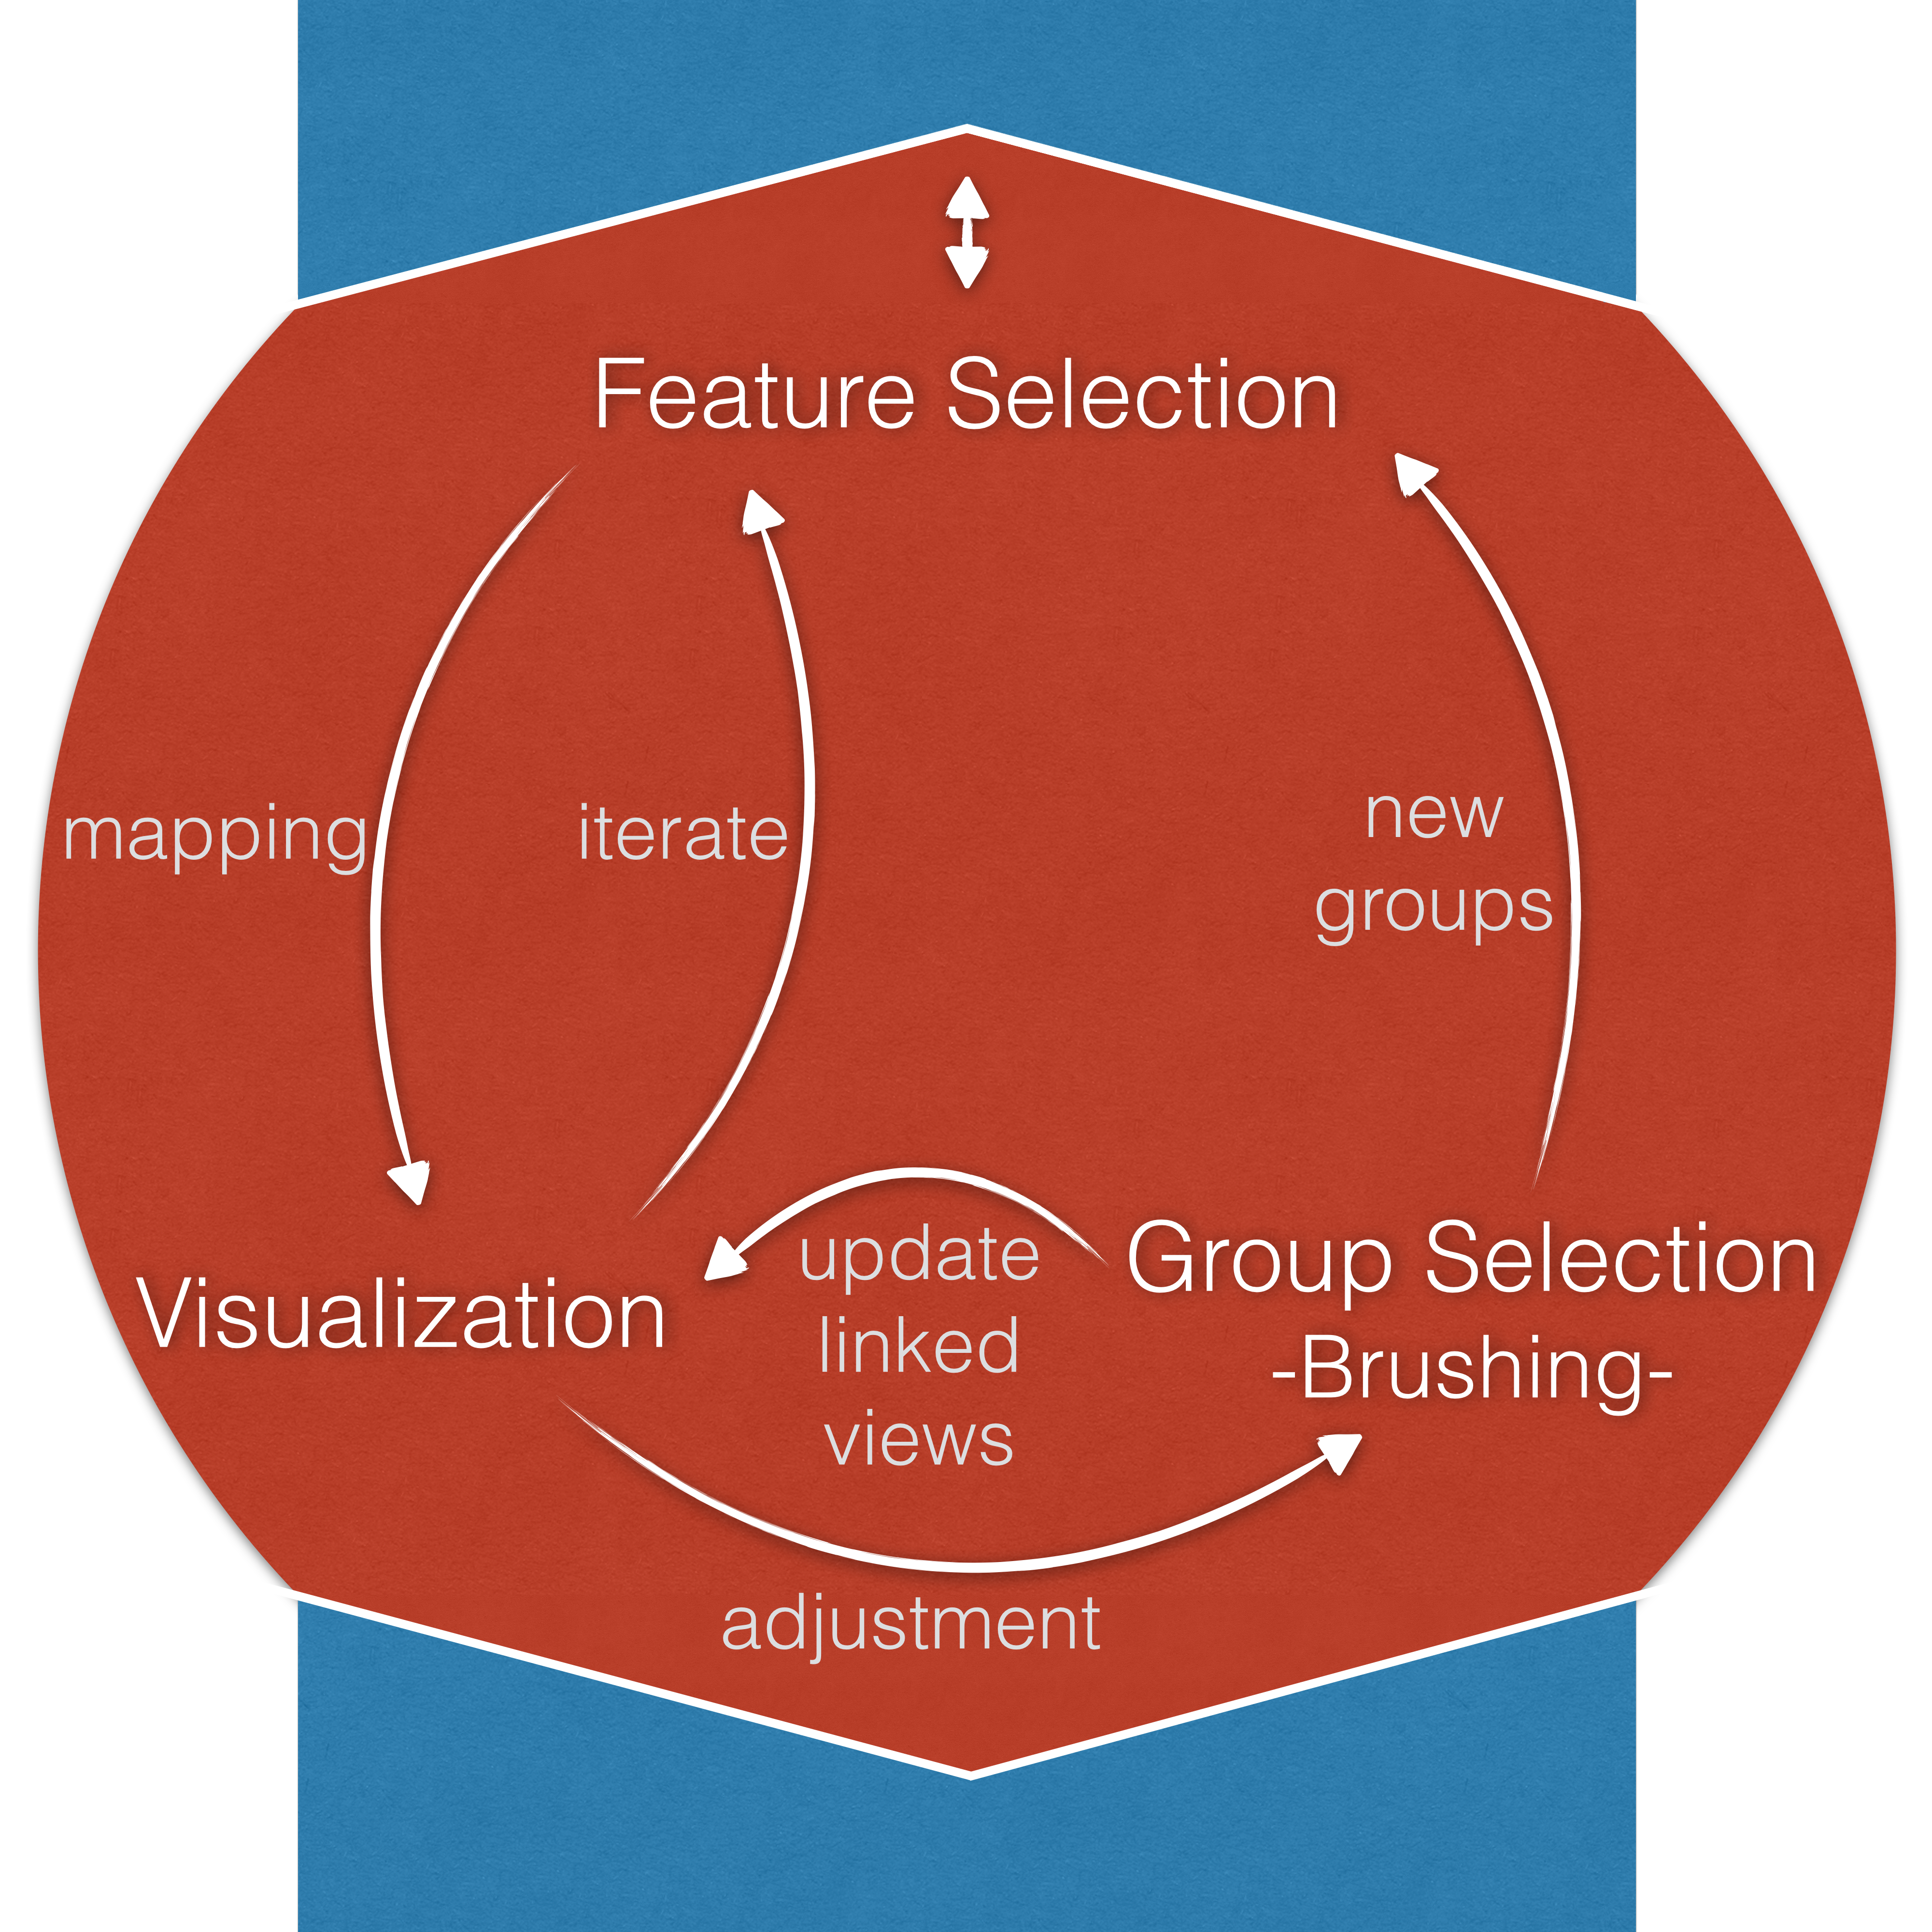
\includegraphics[width=1.5in]{figures/InteractionLoop}
 \includegraphics[width=3.5in]{figures/placeholder}
 \caption{\emph{Image is not final}. (a) "Did you experience back pain in the past three month" Yes No; (b) Clustering of Yes}
 \label{fig:hypopthesisbased}
\end{figure}
%
If the user has already a hypothesis about a relation between a non-image feature regarding shape the workflow slightly differs from the hypothesis free analysis.
%
The starting point of the analysis is the selection of a feature of interest by dragging it into the canvas area and view the subjects distribution as well as their shape differences.
%
In our use case, the epidemiologist was interested in the questionnaire answer "Did you experience back pain in the past three month".
%
The mean shapes of the resulting visualization as seen in Figure~\ref{fig:hypopthesisbased} (a) show no difference between the two groups.
%
Either there are no differences or the variance information was lost in the mean-shape calculation.
%
Since the focus is on subjects which suffer from back pain, the clustering result of these subjects are then drawn into the canvas area, yielding six cluster as seen in Figure~\ref{fig:hypopthesisbased} (b).
%
Cluster 5 stood out for having a so-called hyperlordosis, a strong curvature of the lumbar spine which is a indicator for back pain.

\emph{Cram\'{e}rs' V} contingency values highlighted relationships of this cluster with joint degeneration, meat eating habits, preoccupation, back pain, neck or shoulder pain and waist circumference.
%
Since the prior selection only yields subjects that report back pain, the pain indicators specify the pain localization for the subjects.

It is well known that overweight is a indicator for back pain.
%
While the Body Mass Index (BMI) is a key figure for assessing height and weight of a subject, it does not tell us anything on how the weight is distributed in the body.
%
Our clinical partner were interested in the fact that this group presented a correlation with waist circumference.
%
Our finding follows the recent trends that indicate that BMI is not a good measure for assessing body-shape since healthy weight is dependent on many other measures \cite{Ahima2013}.
%
It indicates that waist circumference rather than the BMI interacts with unusual shaped spines for subjects with lumbar back pain.
%
The influence of the parameter is now in the focus of further analysis.

\subsubsection{Follow-Up Tasks and Concluding Domain-Expert Feedback}
Defining a causal relationship solely based on observed correlations of two features is \emph{cum hoc ergo propter hoc}--correlation does not automatically imply causation \cite{Tufte2003}.
%
The observed correlations need to be carefully checked for confounder and medical soundness!
%
Statisticians validate causal inferences of the drawn conclusions.

Features that potentially interact with a disease related condition need to be validated.
%
To increase the probability of the observation not to be random, our clinical partners cross check for interactions in another cohort, the \texttt{SHIP-TREND}.
%If features are identified as interesting for a disease, the epidemiologists look for interactions in another cohort, the \texttt{SHIP-TREND}.
%
%If the correlation is observed there as well, it is likely not random.
\\\\
Our clinical partners pointed out the usability of the presented methods to guide their attention to features which where not in the focus of their attention and expectance.
%
The explorative nature of the methods work well for gathering interactions which may act as confounder, as outcome of a disease or as an actual cause or risk factor.
%"\emph{Correlation does not imply causation}" is a famous saying in statistics, meaning that correlation does not necessarily imply causal relationships \cite{}.
%
This distinction is hard to make and requires a lot of clinical experience.
%
The combination of multiple views with shape information help to connect many different information sources to make the large information spaces cognitive feasible.
%

On the feature level, our clinical partners were interested in the MRI scans for the subjects in the outlier clusters because they are highly likely to exhibit pathologies.
%
We plan to include a \texttt{DICOM}-viewer to meet this wish.

% - Describe steps from gathering Information from the raw image files (segmentation, abstraction, visualization)\\
% - Problem of sparse differences - Visualization has to be more abstract to emphasize the differences.\\
% - Input of Epidemiologists goes here!\\

\section{Summary and Conclusion}
- Future Work: Matrix-View of differences - more intuitive\\
- UI more flexible by hiding UI-panes
- Dynamic Discretization to better fit the data distributions
- More Shape based filtering - reorder by size, curvature, etc. ...
- Color code different Aspects - Only difference in x or y direction
- Calculation of contingency based on the contingency differences - how does the current selection differ compared to the whole data set?

Discretization of continuos variables into bins of equal size may bias the underlying data by not considering the variable distribution function \cite{Fletcher2012}.
% Fletcher 2012 - S. 257
To reduce the number of false positive findings, the data space can be randomly be cut in half the hypothesis then can be cross-validated for statistical soundness.
%
This requires a large number of subjects, especially if the investigated features are rare and are only presented by a few subjects.
%
As suggested by Fletcher and Fletcher, we plan to validate the hypothesis using the \texttt{SHIP-TREND} cohort \cite{Fletcher2012}.


%% if specified like this the section will be committed in review mode
%\acknowledgments{SHIP is part of the Community Medicine Research net of the University of Greifswald, Germany, which is funded by the Federal Ministry of Education and Research (grant no. 03ZIK012), the Ministry of Cultural Affairs as well as the Social Ministry of the Federal State of Mecklenburg-West Pomerania. Whole-body MR imaging was supported by a joint grant from Siemens Healthcare, Erlangen, Germany and the Federal State of Mecklenburg-Vorpommern. The University of Greifswald is a member of the ‘Centre of Knowledge Interchange’ program of the Siemens AG. This work was supported by the DFG Priority Program 1335: Scalable Visual Analytics.}

\bibliographystyle{abbrv}
%%use following if all content of bibtex file should be shown
%\nocite{*}
\bibliography{bibliography}
\end{document}
